\section{测试}
\subsection{业务逻辑层服务}
业务逻辑层服务众多,如第四章介绍的,但测试流程基本上相同,这里只拿典型举例:
\subsubsection{获取车站布局测试}
测试输入(其中的实例id是之前创建的):
\begin{lstlisting}
query {
  stationLayout(id: "db42f0ed-d096-4805-b048-909e69dd44e2") {
    title,
    nodes{
      nodeId, 
      trackId, 
      leftP{x,y}, 
      rightP{x,y}, 
      leftJoint, 
      rightJoint
    },
    signals{
      signalId,
      sgnType,
      sgnMnt,
      protectNodeId,
      side,
      dir,
      pos{x,y},
      btns
    }
  }
}
\end{lstlisting}

服务输出:
\begin{lstlisting}
{
  "data": {
    "stationLayout": {
      "nodes": [
        {
          "leftJoint": "EMPTY",
          "leftP": {
            "x": 0,
            "y": 5
          },
          "nodeId": 1,
          "rightJoint": "NORMAL",
          "rightP": {
            "x": 5,
            "y": 5
          },
          "trackId": "X3JG"
        },
        {
          "leftJoint": "NORMAL",
          "leftP": {
            "x": 5,
            "y": 5
          },
          "nodeId": 5,
          "rightJoint": "NORMAL",
          "rightP": {
            "x": 5,
            "y": 10
          },
          "trackId": "IAG"
        }
      ],
      "signals": [
        {
          "btns": [
            "PASS",
            "GUIDE",
            "TRAIN"
          ],
          "dir": "LEFT",
          "pos": {
            "x": 5,
            "y": 5
          },
          "protectNodeId": 5,
          "sgnMnt": "POST_MOUNTING",
          "sgnType": "HOME_SIGNAL",
          "side": "UPPER",
          "signalId": "X"
        }
      ],
      "title": "测试站"
    }
  }
}
\end{lstlisting}
\subsection{控制台界面}
\begin{figure}[htbp!]
  \centering
  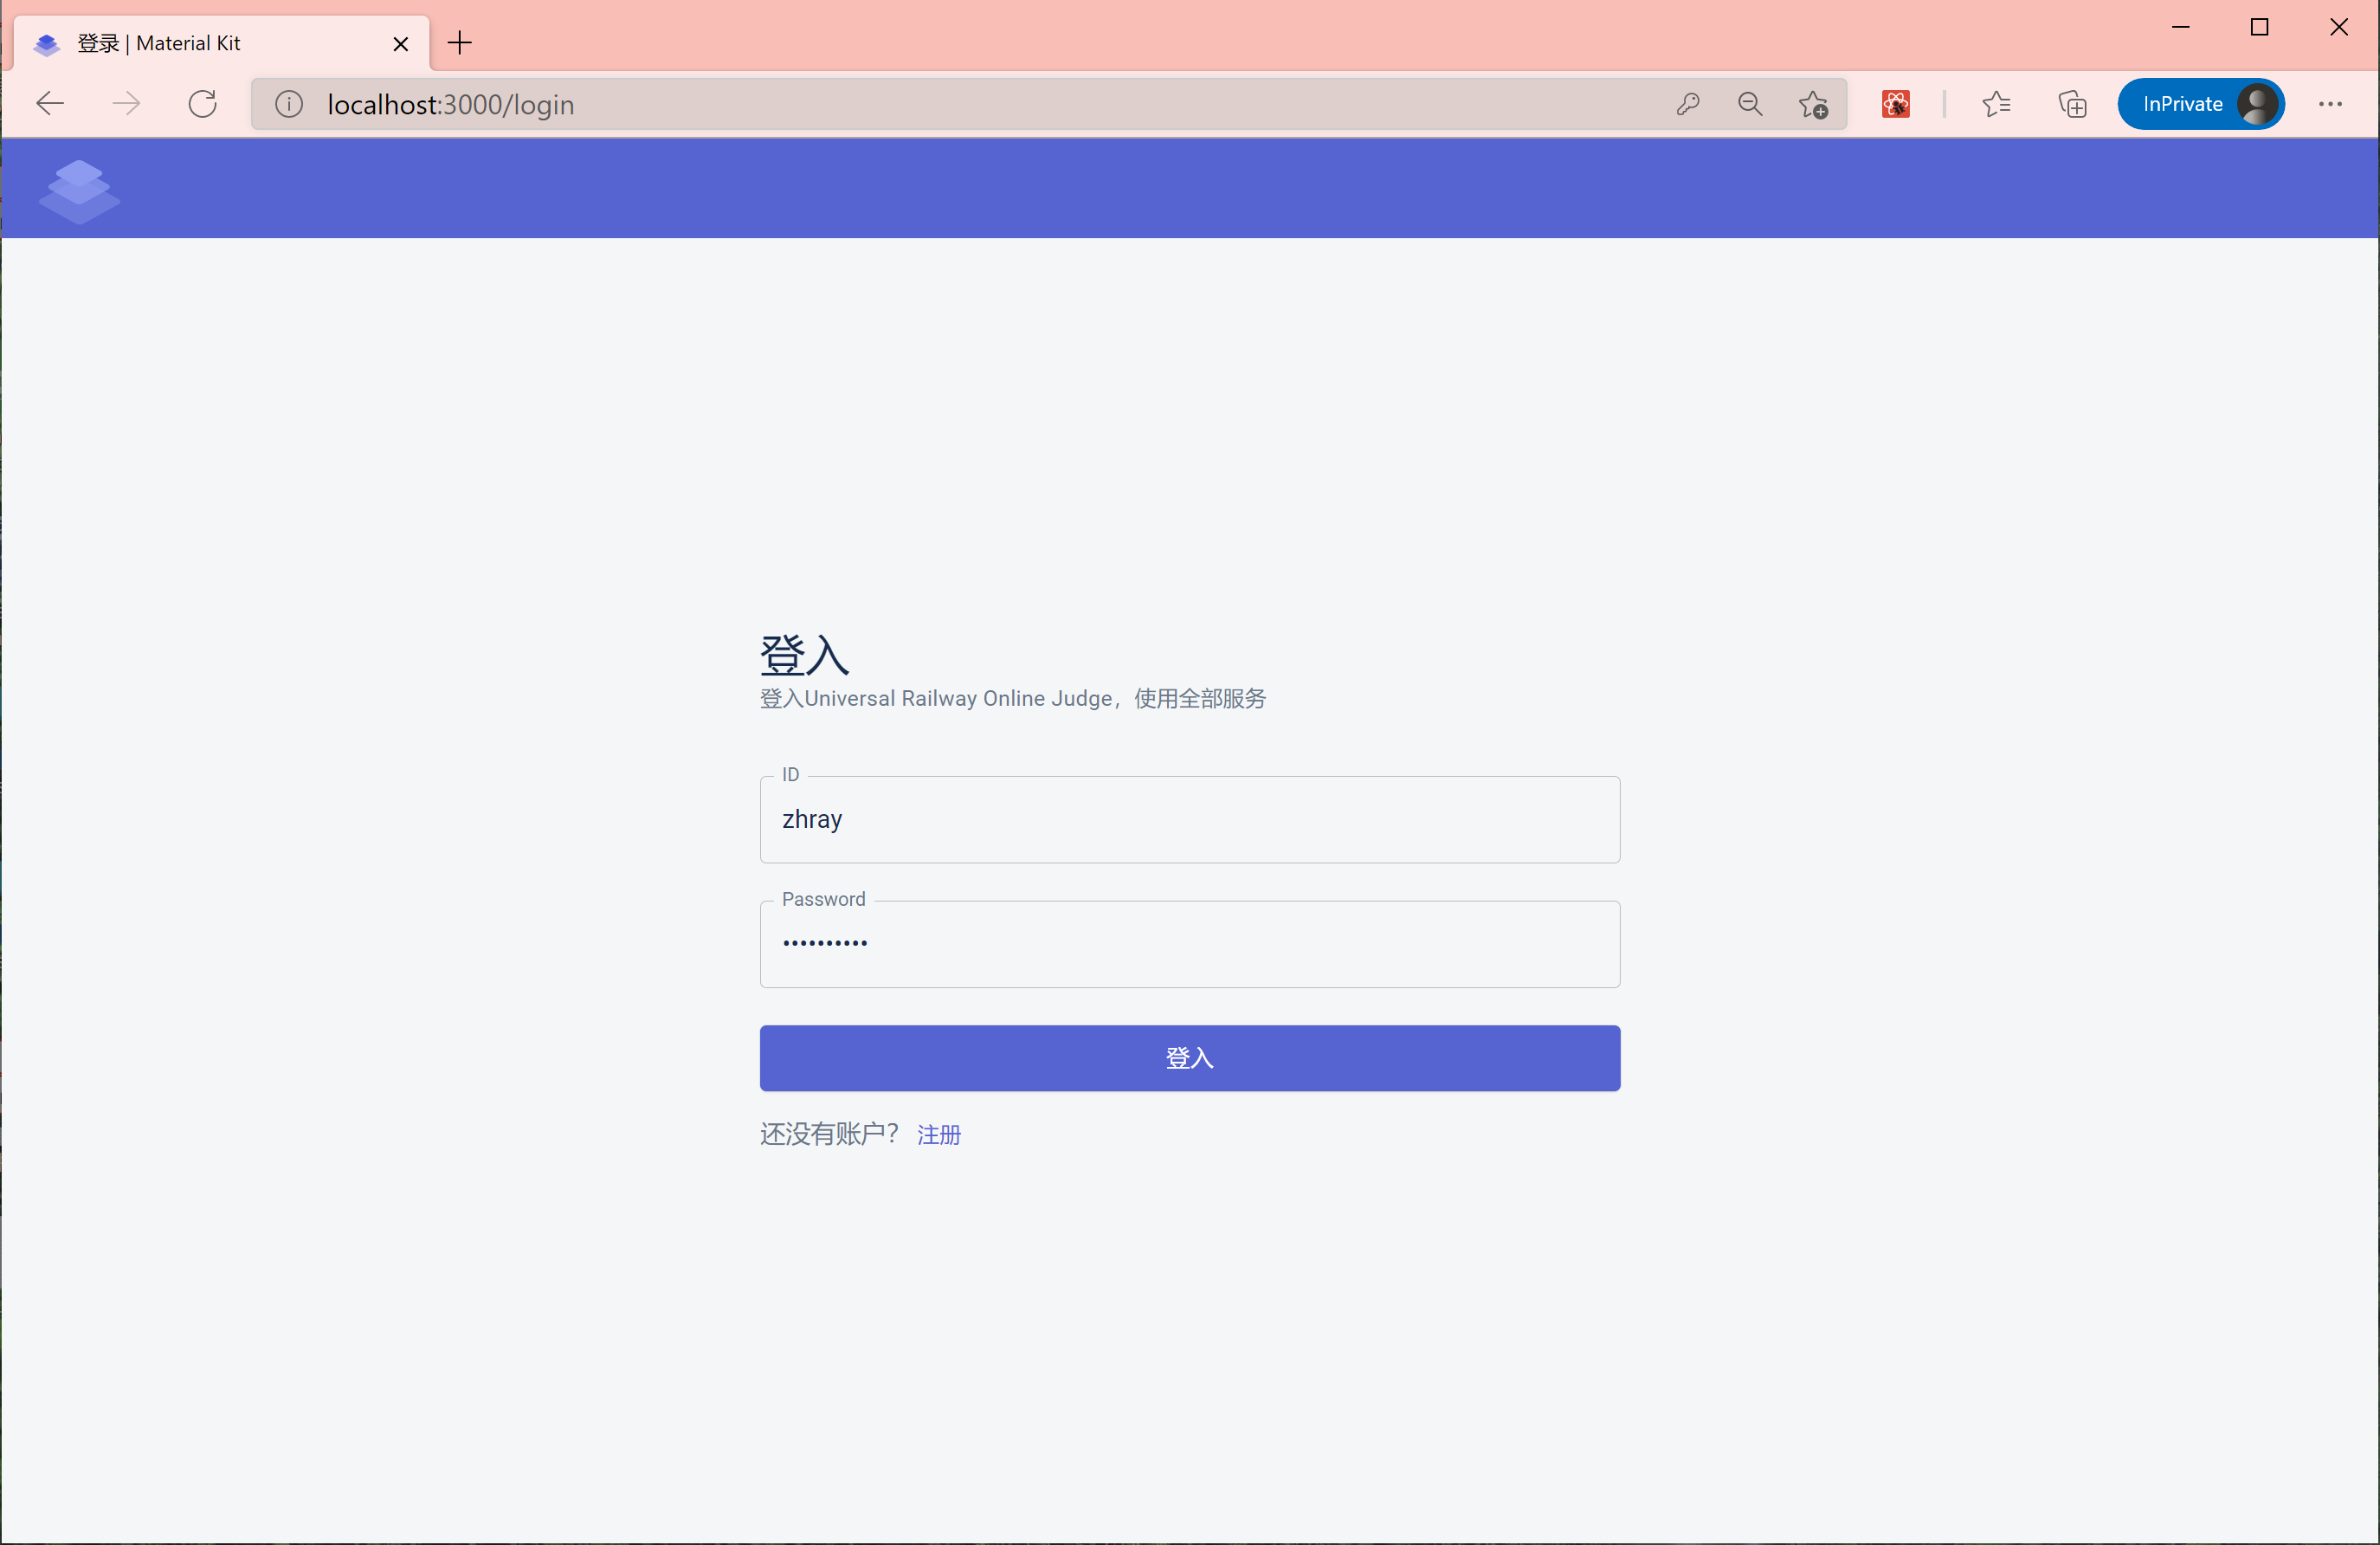
\includegraphics[width=\textwidth]{figures/png/login.png}
  \caption{\label{login}登录界面}
\end{figure}

登录界面如图\ref{login} 所示,当登录成功后,系统会跳转页面至控制台。
如果登陆失败则会报错

\begin{figure}[htbp!]
  \centering
  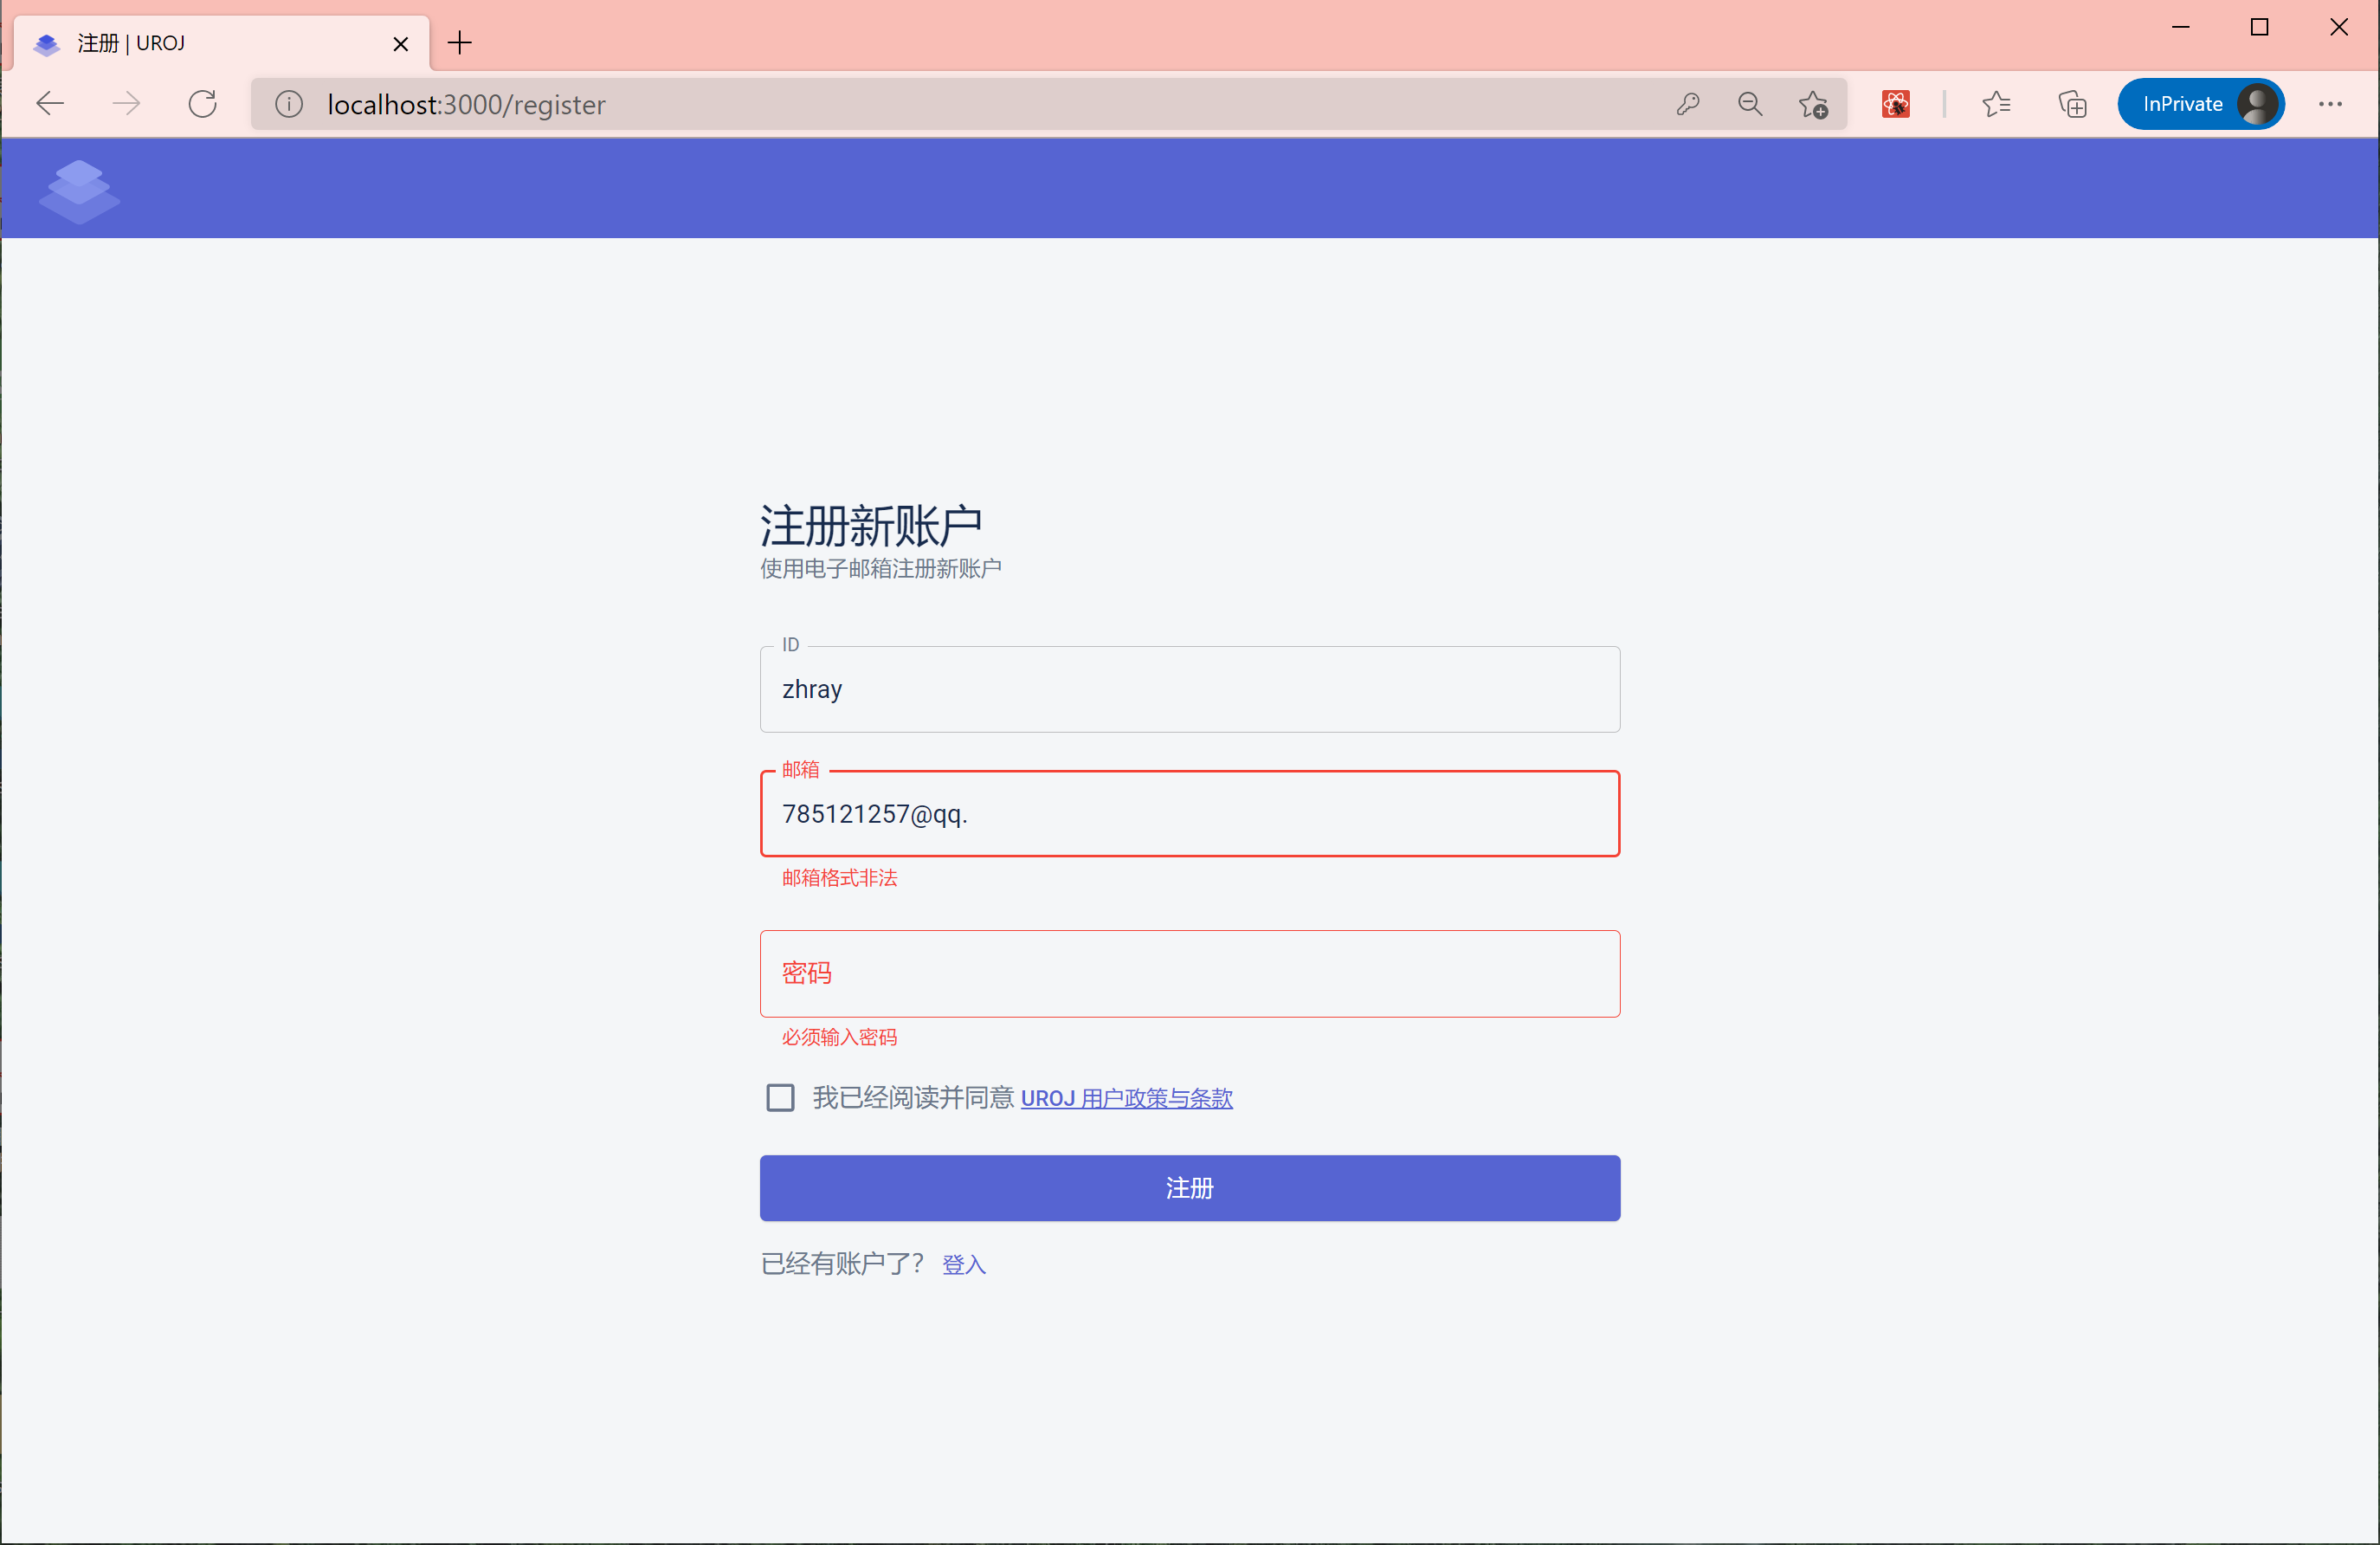
\includegraphics[width=\textwidth]{figures/png/input_err.png}
  \caption{\label{input_err}注册}
\end{figure}

注册界面如图\ref{input_err} 所示,当注册成功后,系统会询问是否跳转页面至登录。
如果注册失败则会报错

\begin{figure}[htbp!]
  \centering
  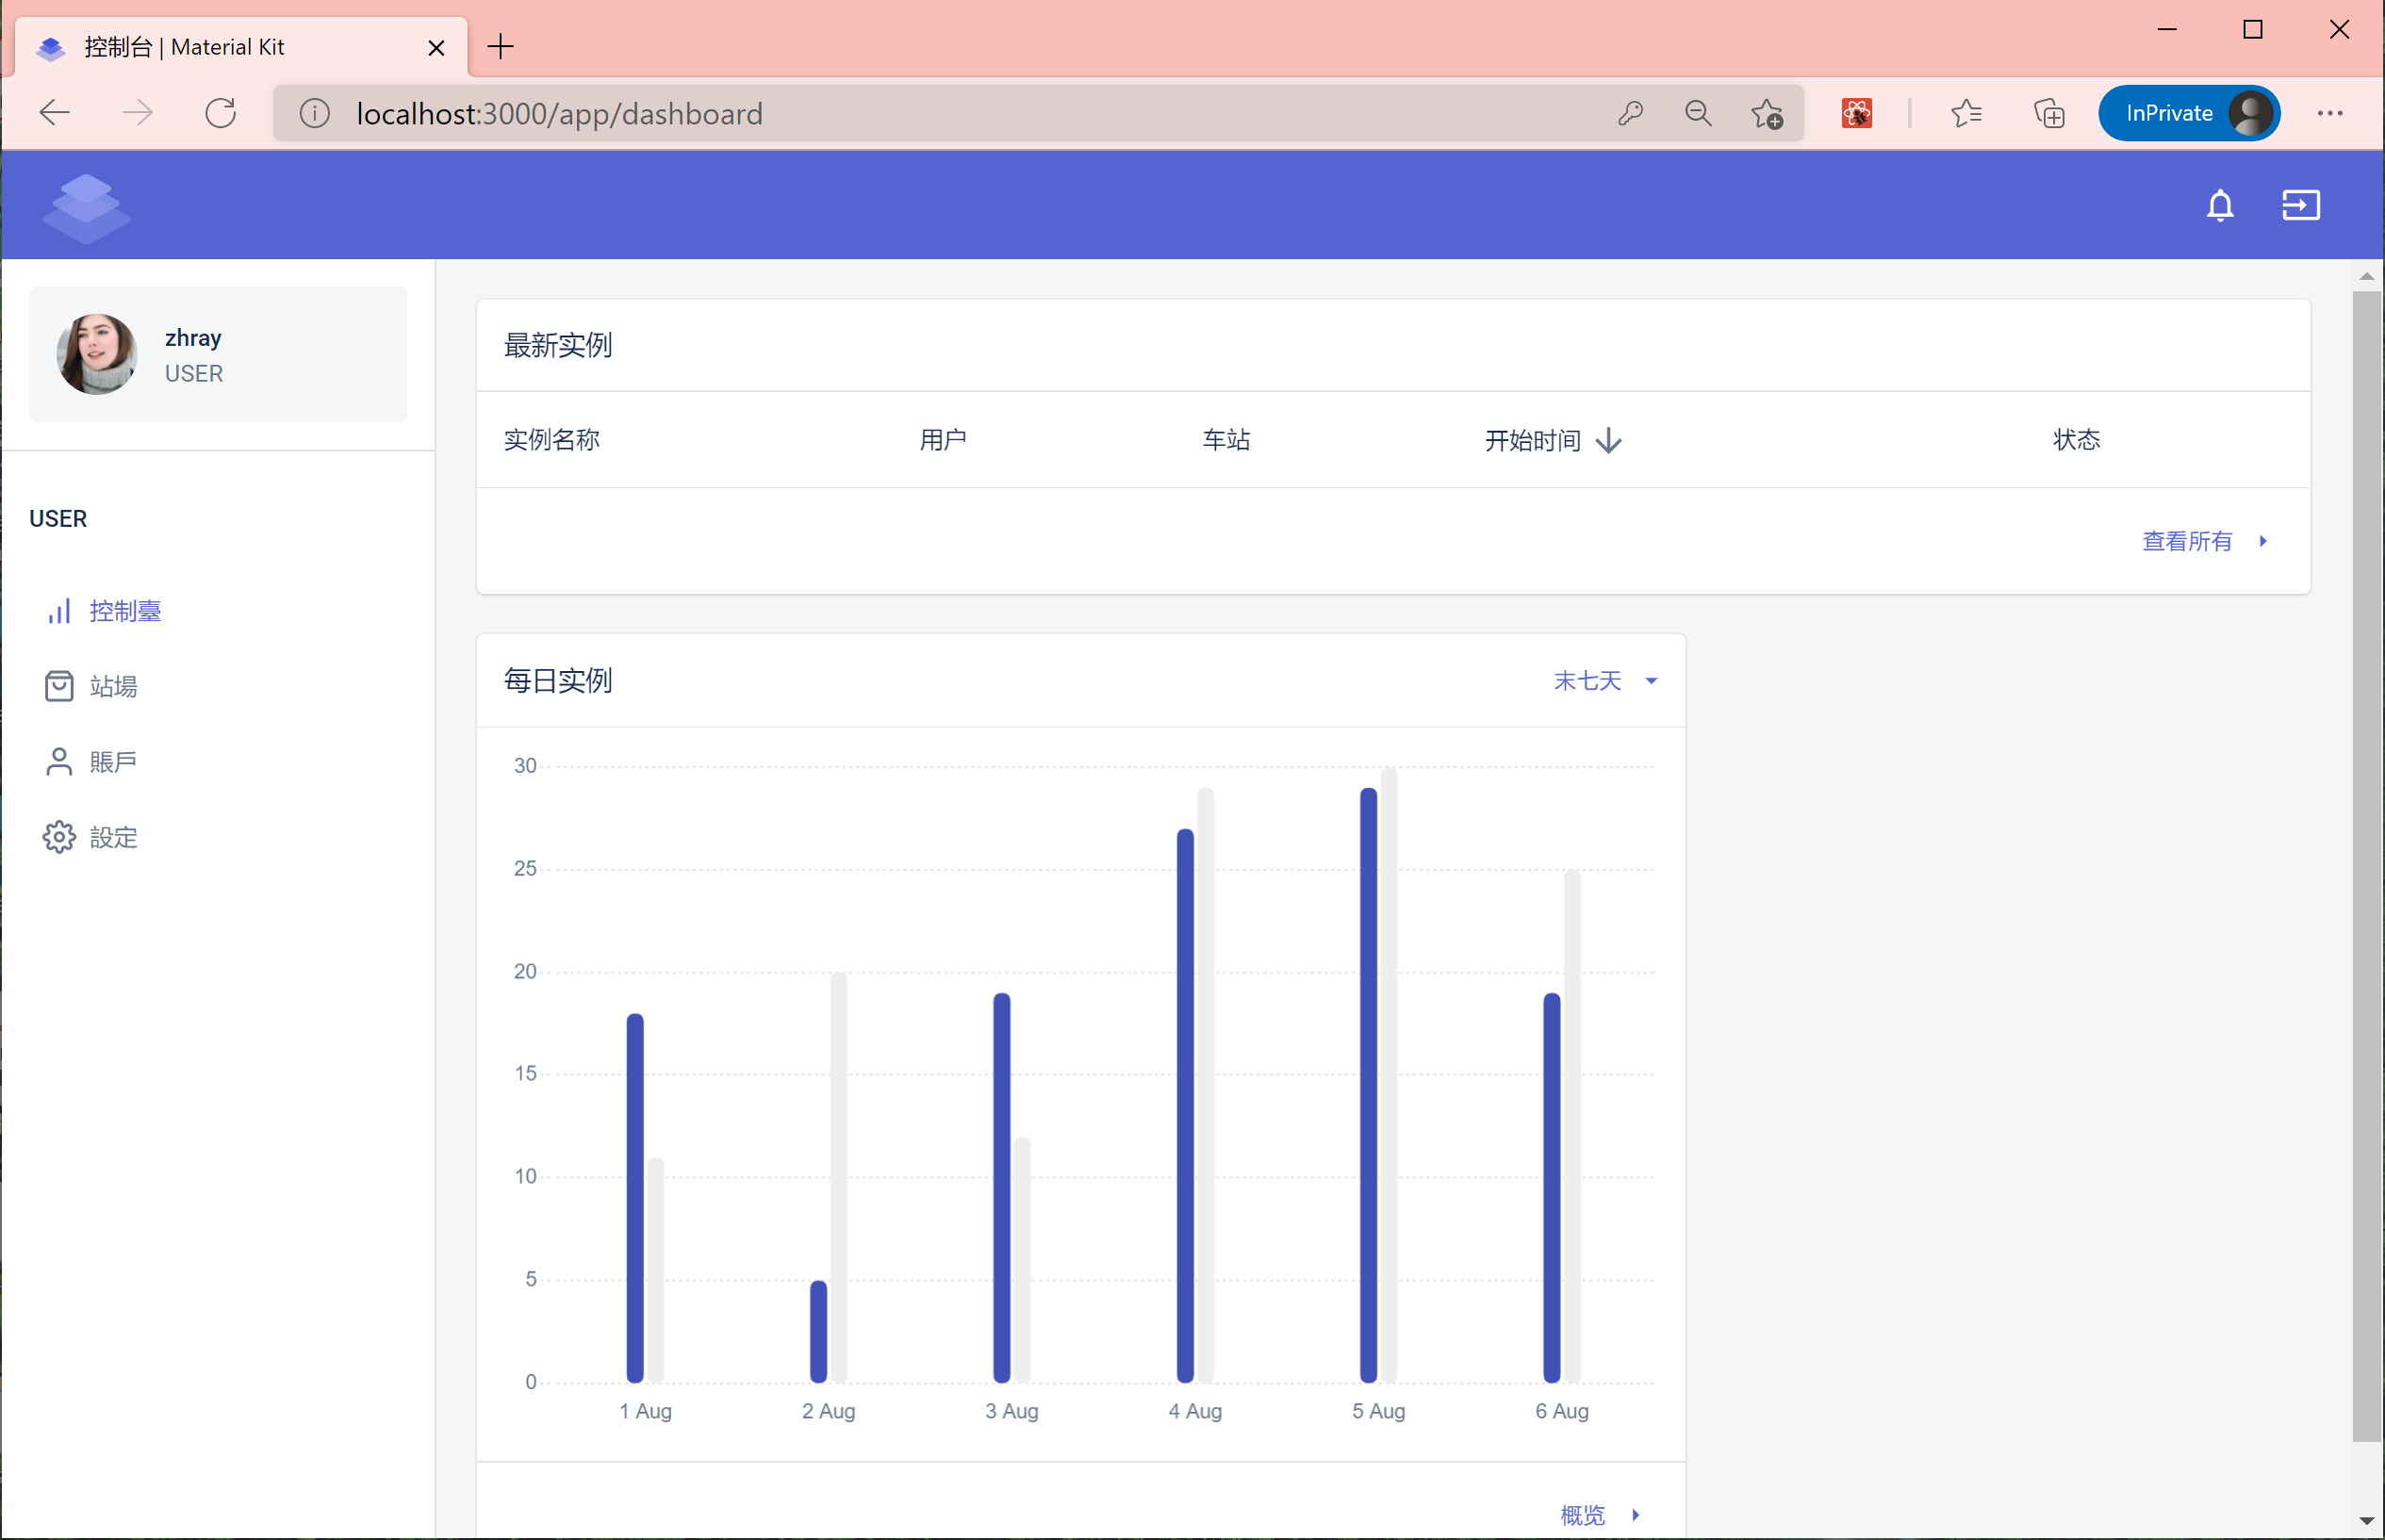
\includegraphics[width=\textwidth]{figures/png/user_ui.png}
  \caption{\label{user_ui}用户角色的控制台首页}
\end{figure}

USER 角色的控制台界面如图\ref{user_ui} 所示,在侧边栏中是可供用户
点入的功能清单。

\begin{figure}[htbp!]
  \centering
  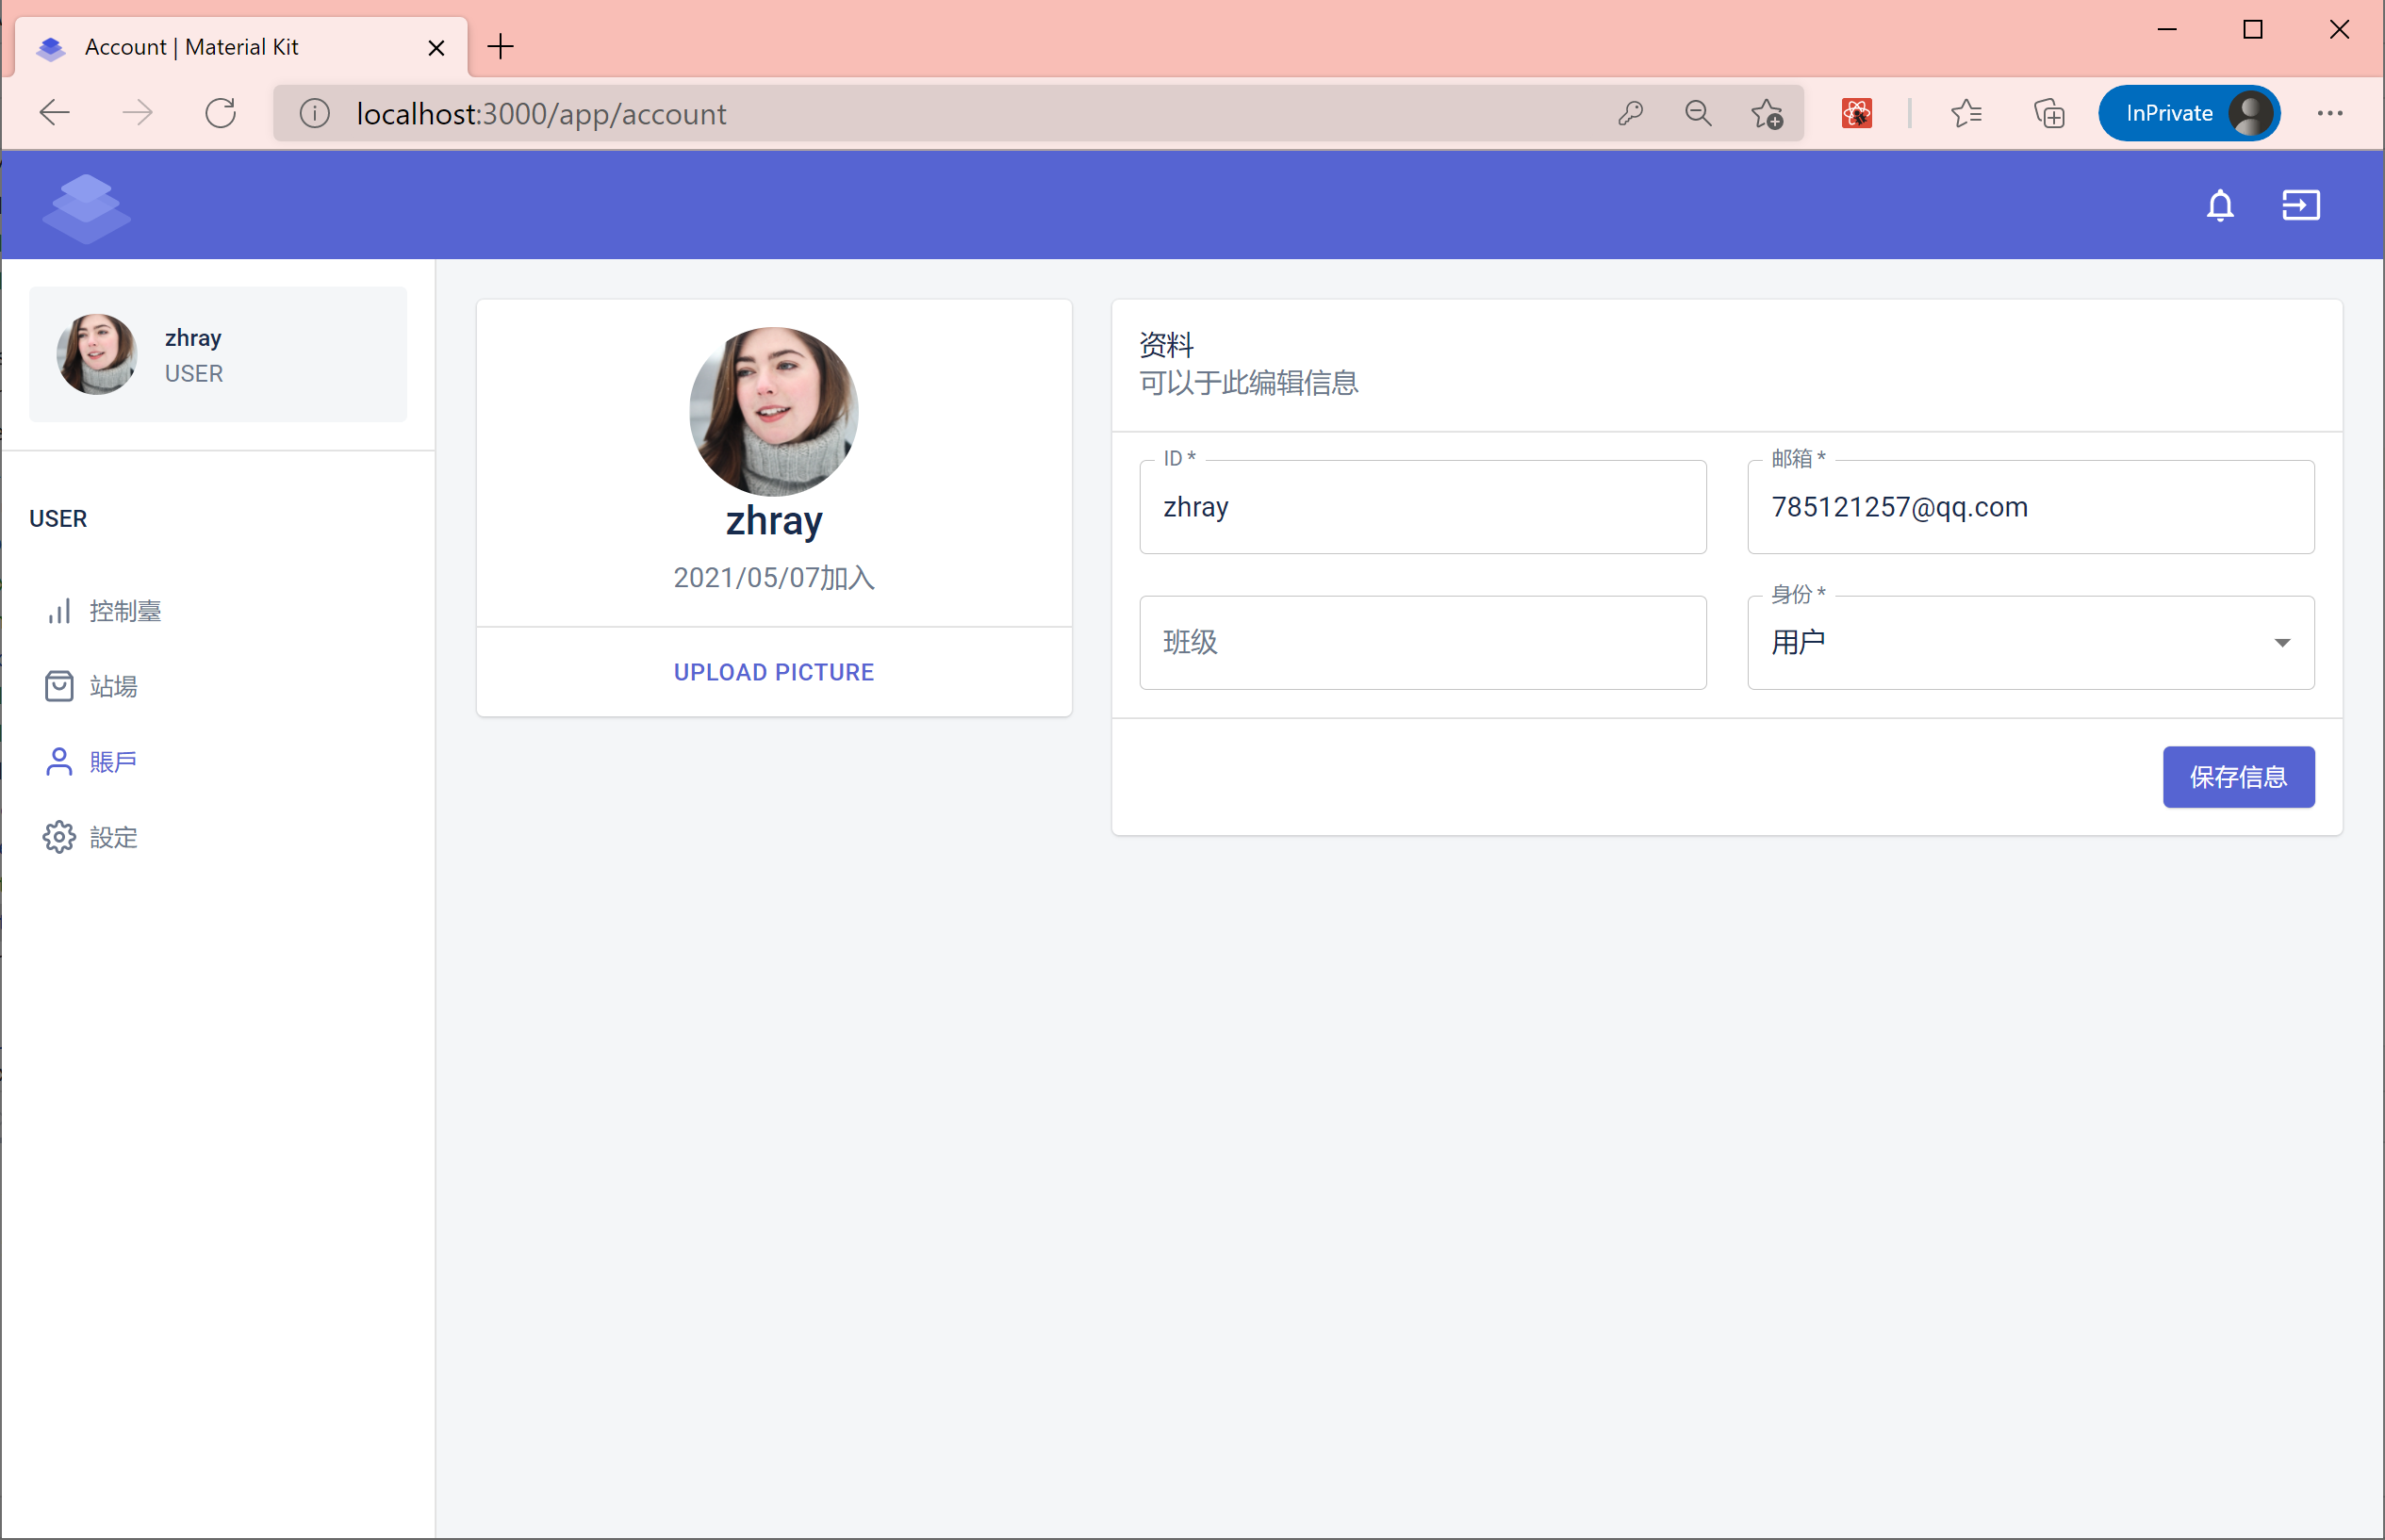
\includegraphics[width=\textwidth]{figures/png/user_data.png}
  \caption{\label{user_data}用户信息页}
\end{figure}

\begin{figure}[htbp!]
  \centering
  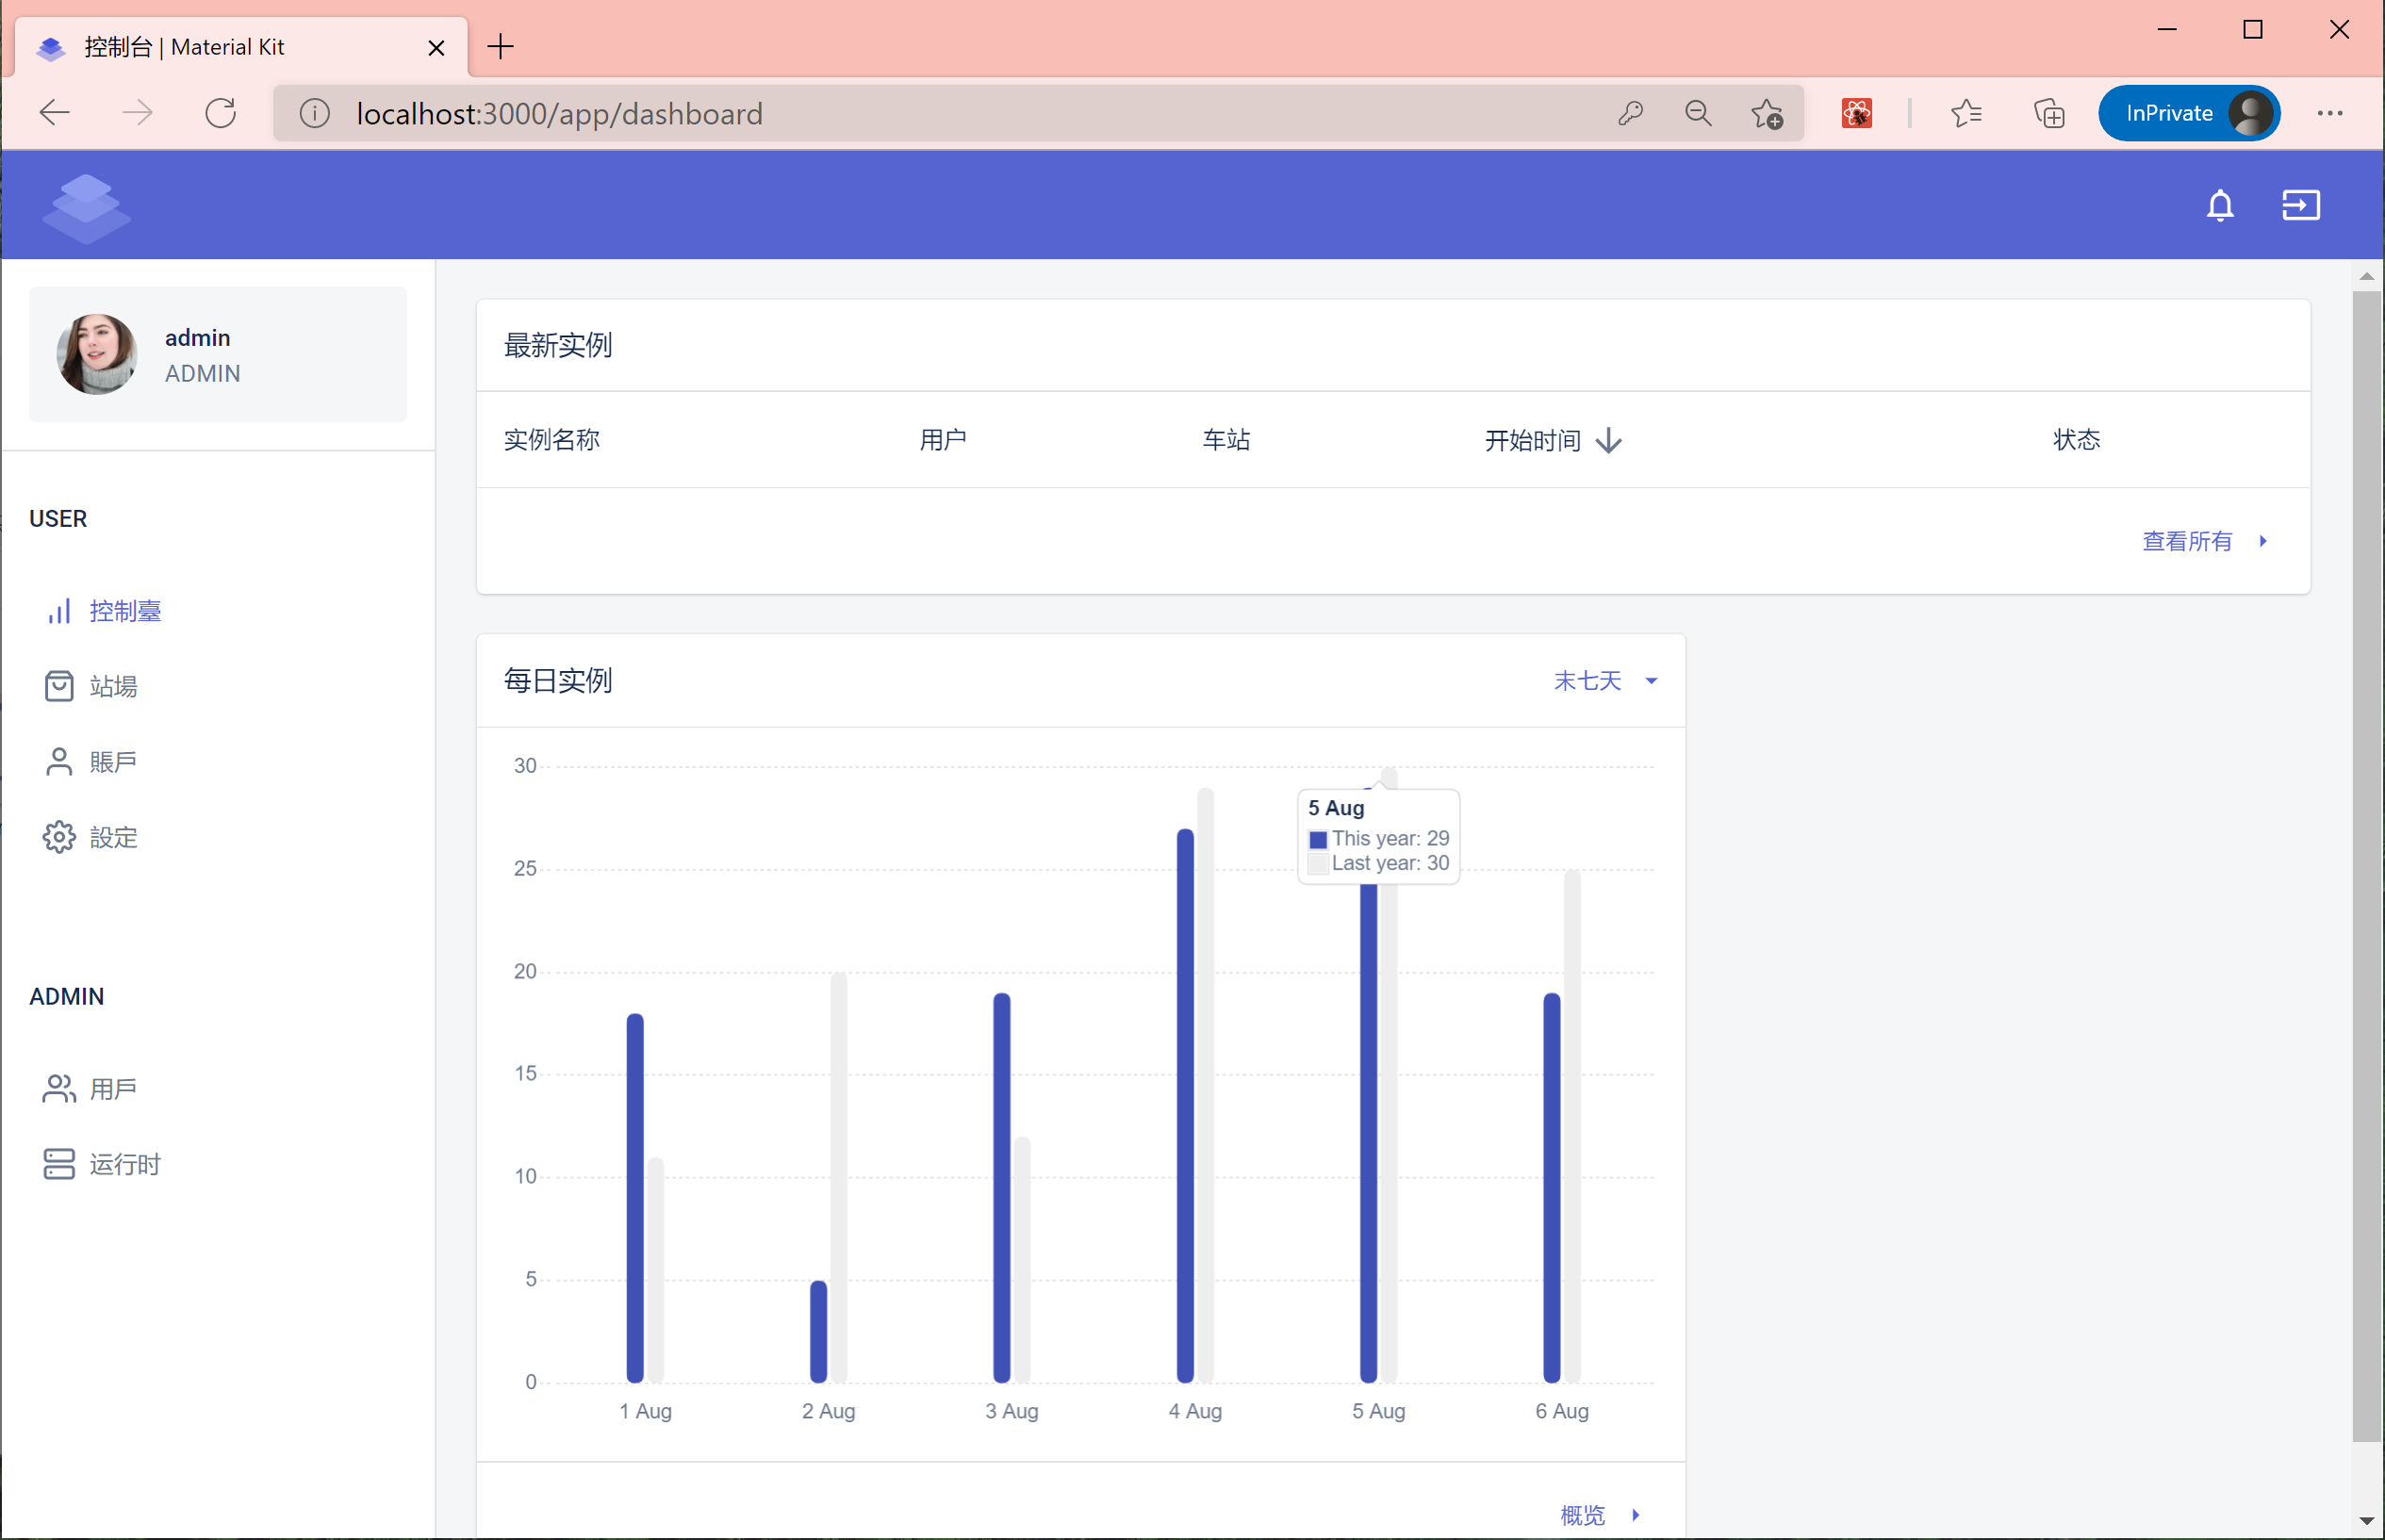
\includegraphics[width=\textwidth]{figures/png/admin_ui.png}
  \caption{\label{admin_ui}管理员角色的控制台首页}
\end{figure}

管理员角色的控制台界面如图\ref{admin_ui} 所示,在侧边栏中是可供用户
点入的功能清单。但与用户角色不同的是,多了用户管理以及运行时管理这两项
只有管理员才有权使用的功能。

\begin{figure}[htbp!]
  \centering
  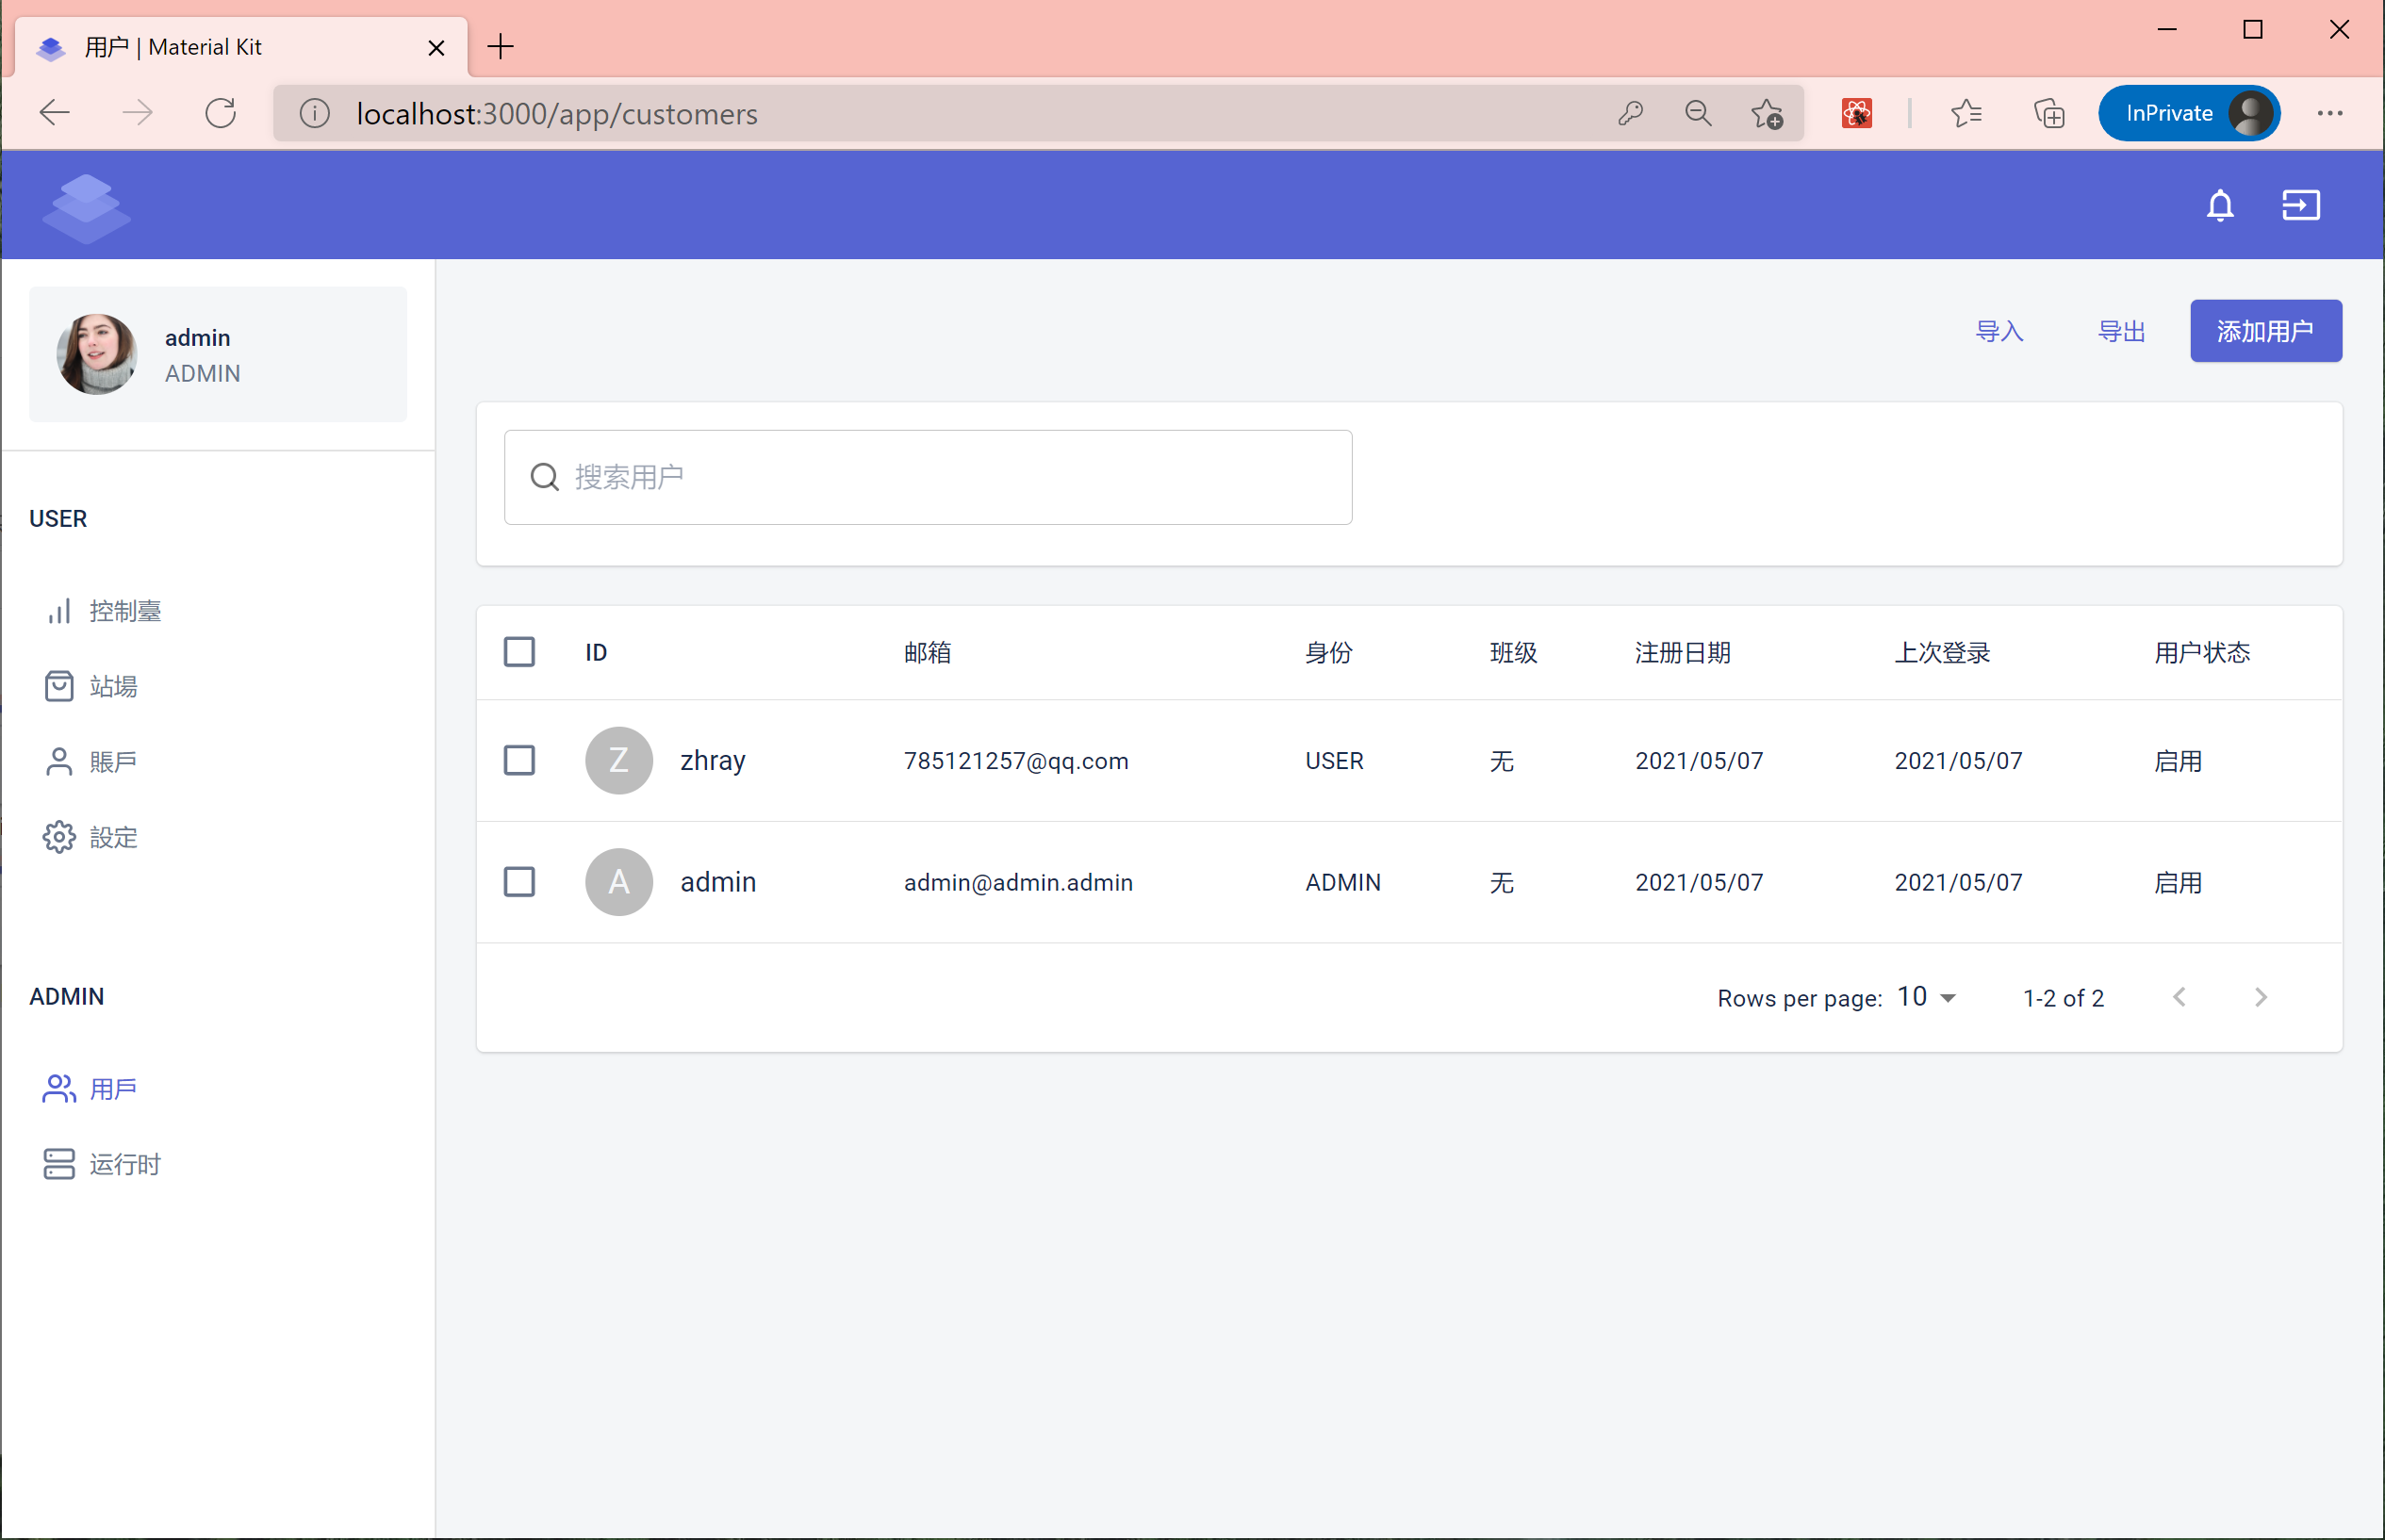
\includegraphics[width=\textwidth]{figures/png/admin_users.png}
  \caption{\label{admin_users}用户管理}
\end{figure}

图\ref{admin_users} 是管理员功能之一的用户管理,从中可以看到刚刚注册成功的zhray账户。

\begin{figure}[htbp!]
  \centering
  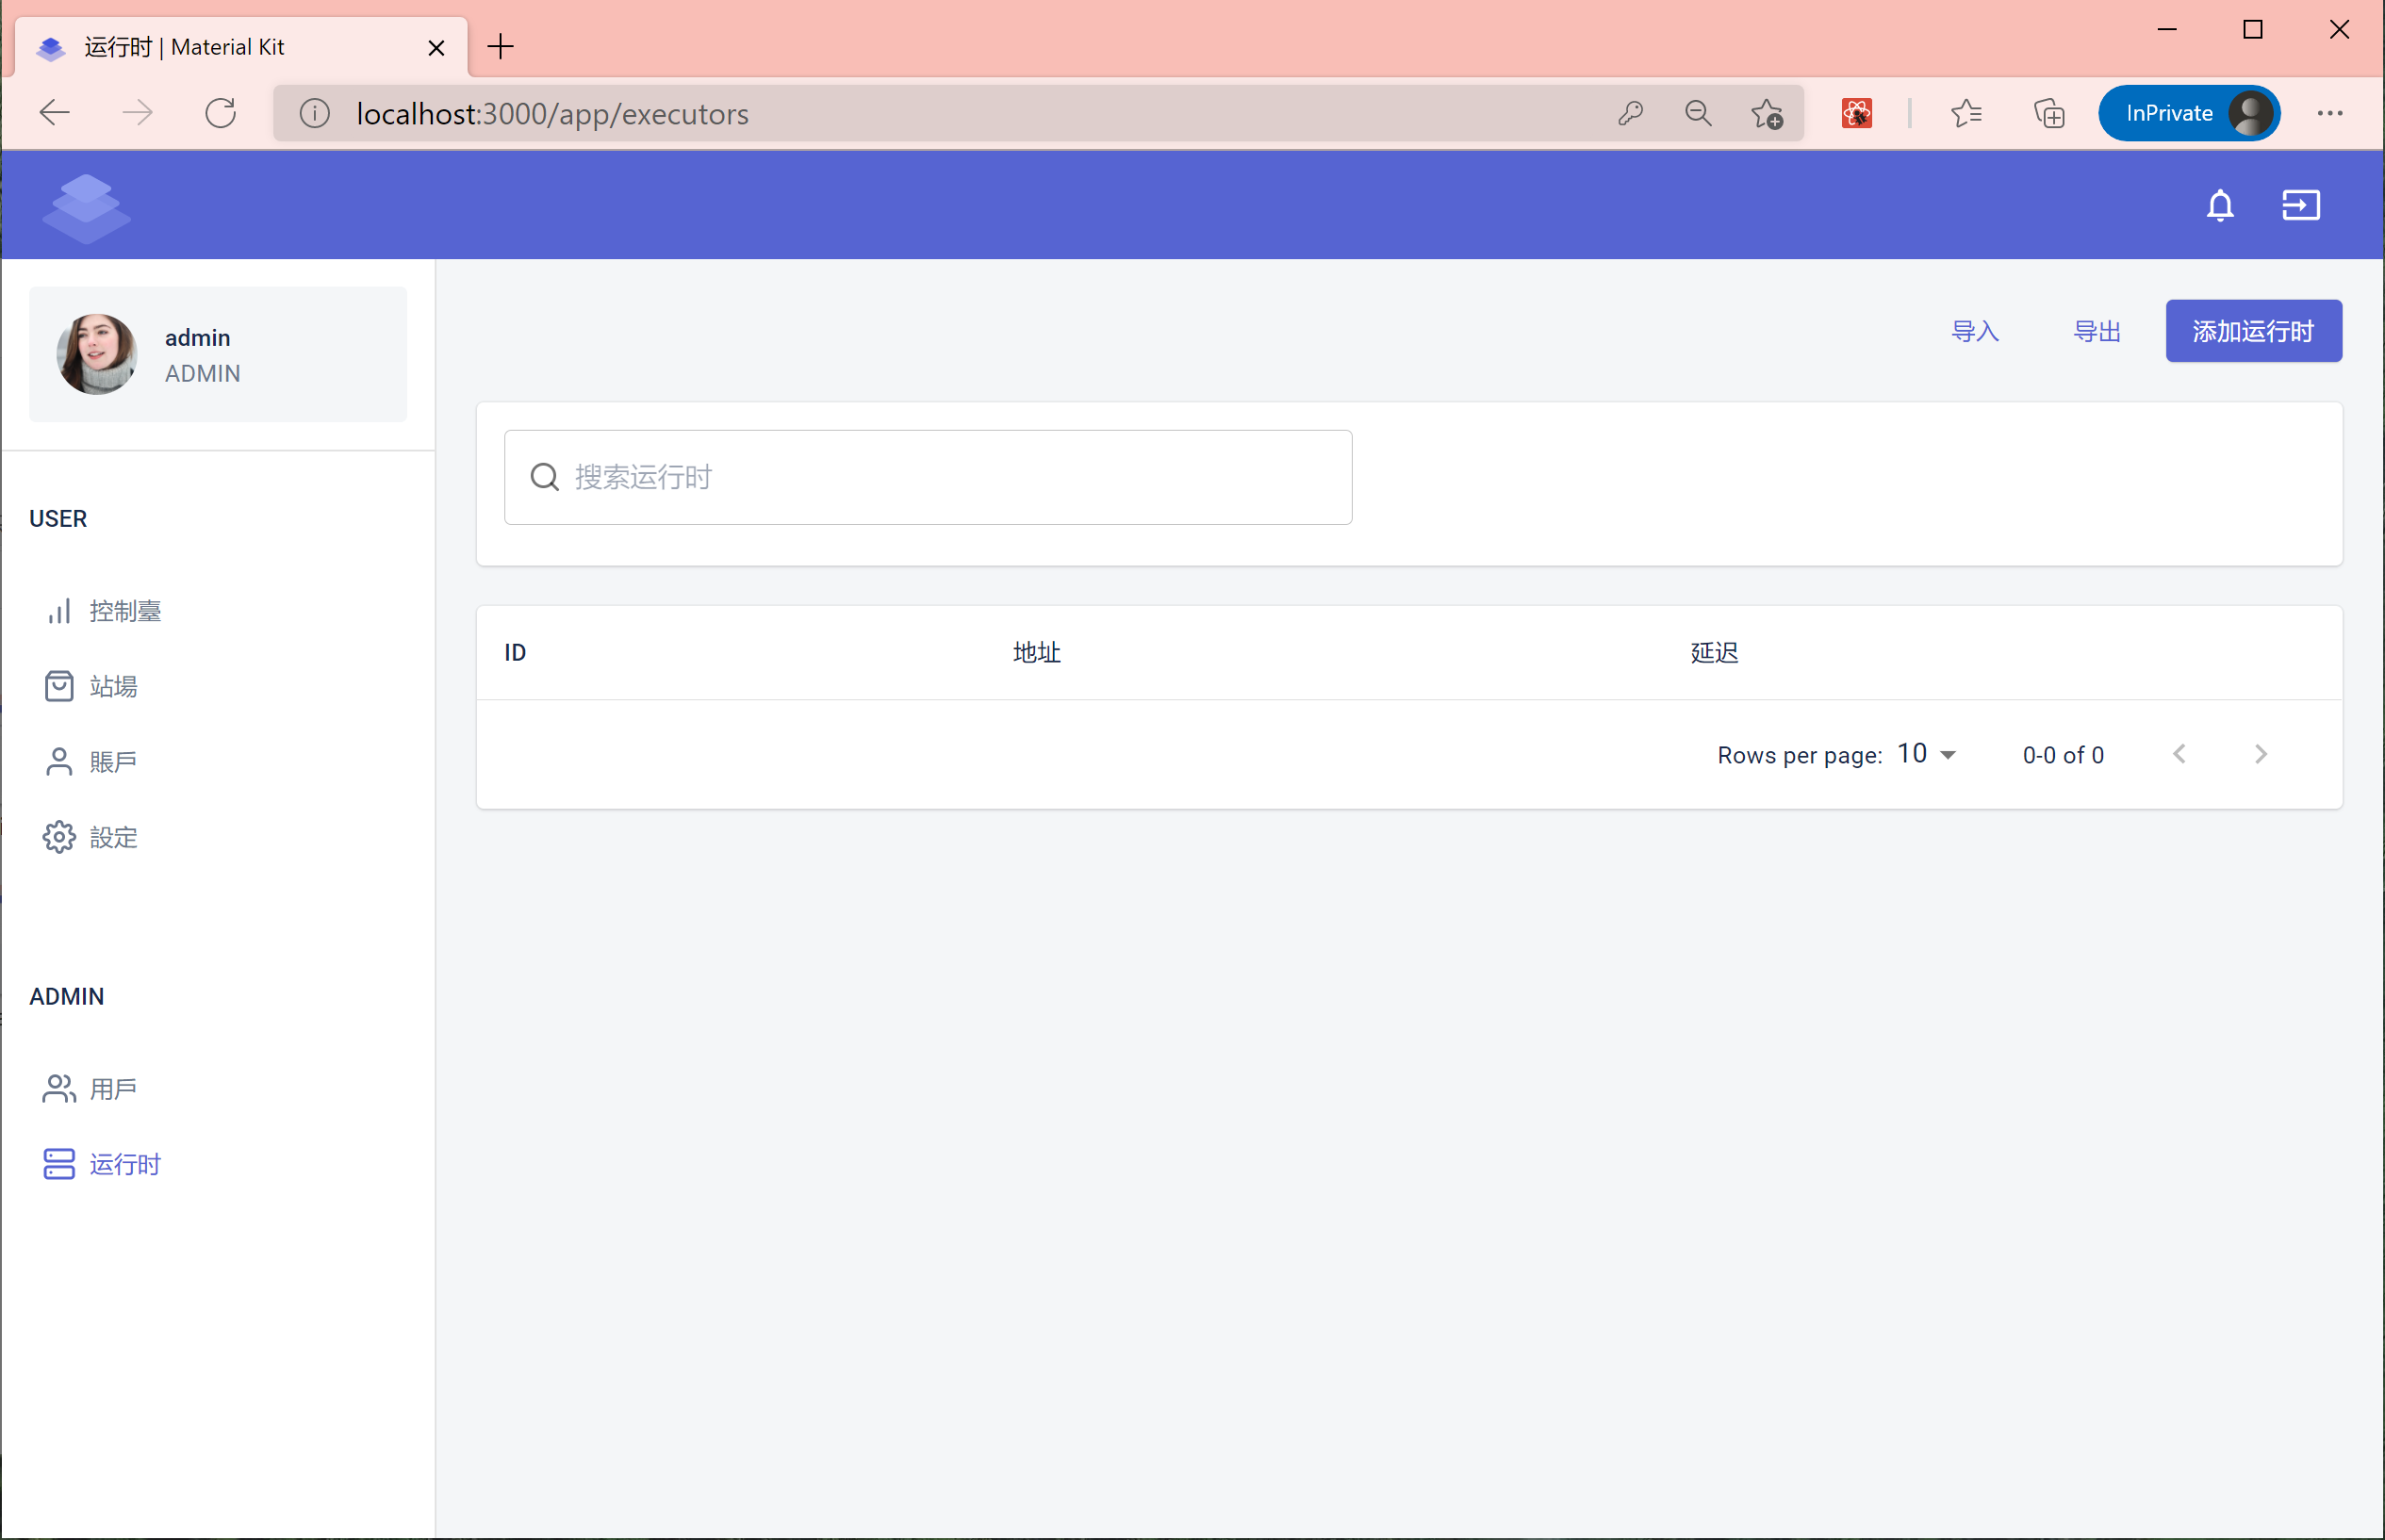
\includegraphics[width=\textwidth]{figures/png/exes.png}
  \caption{\label{exes}运行时管理}
\end{figure}

图\ref{exes} 是管理员功能之一的运行时管理。可以在这里增删改查运行时。

\begin{figure}[htbp!]
  \centering
  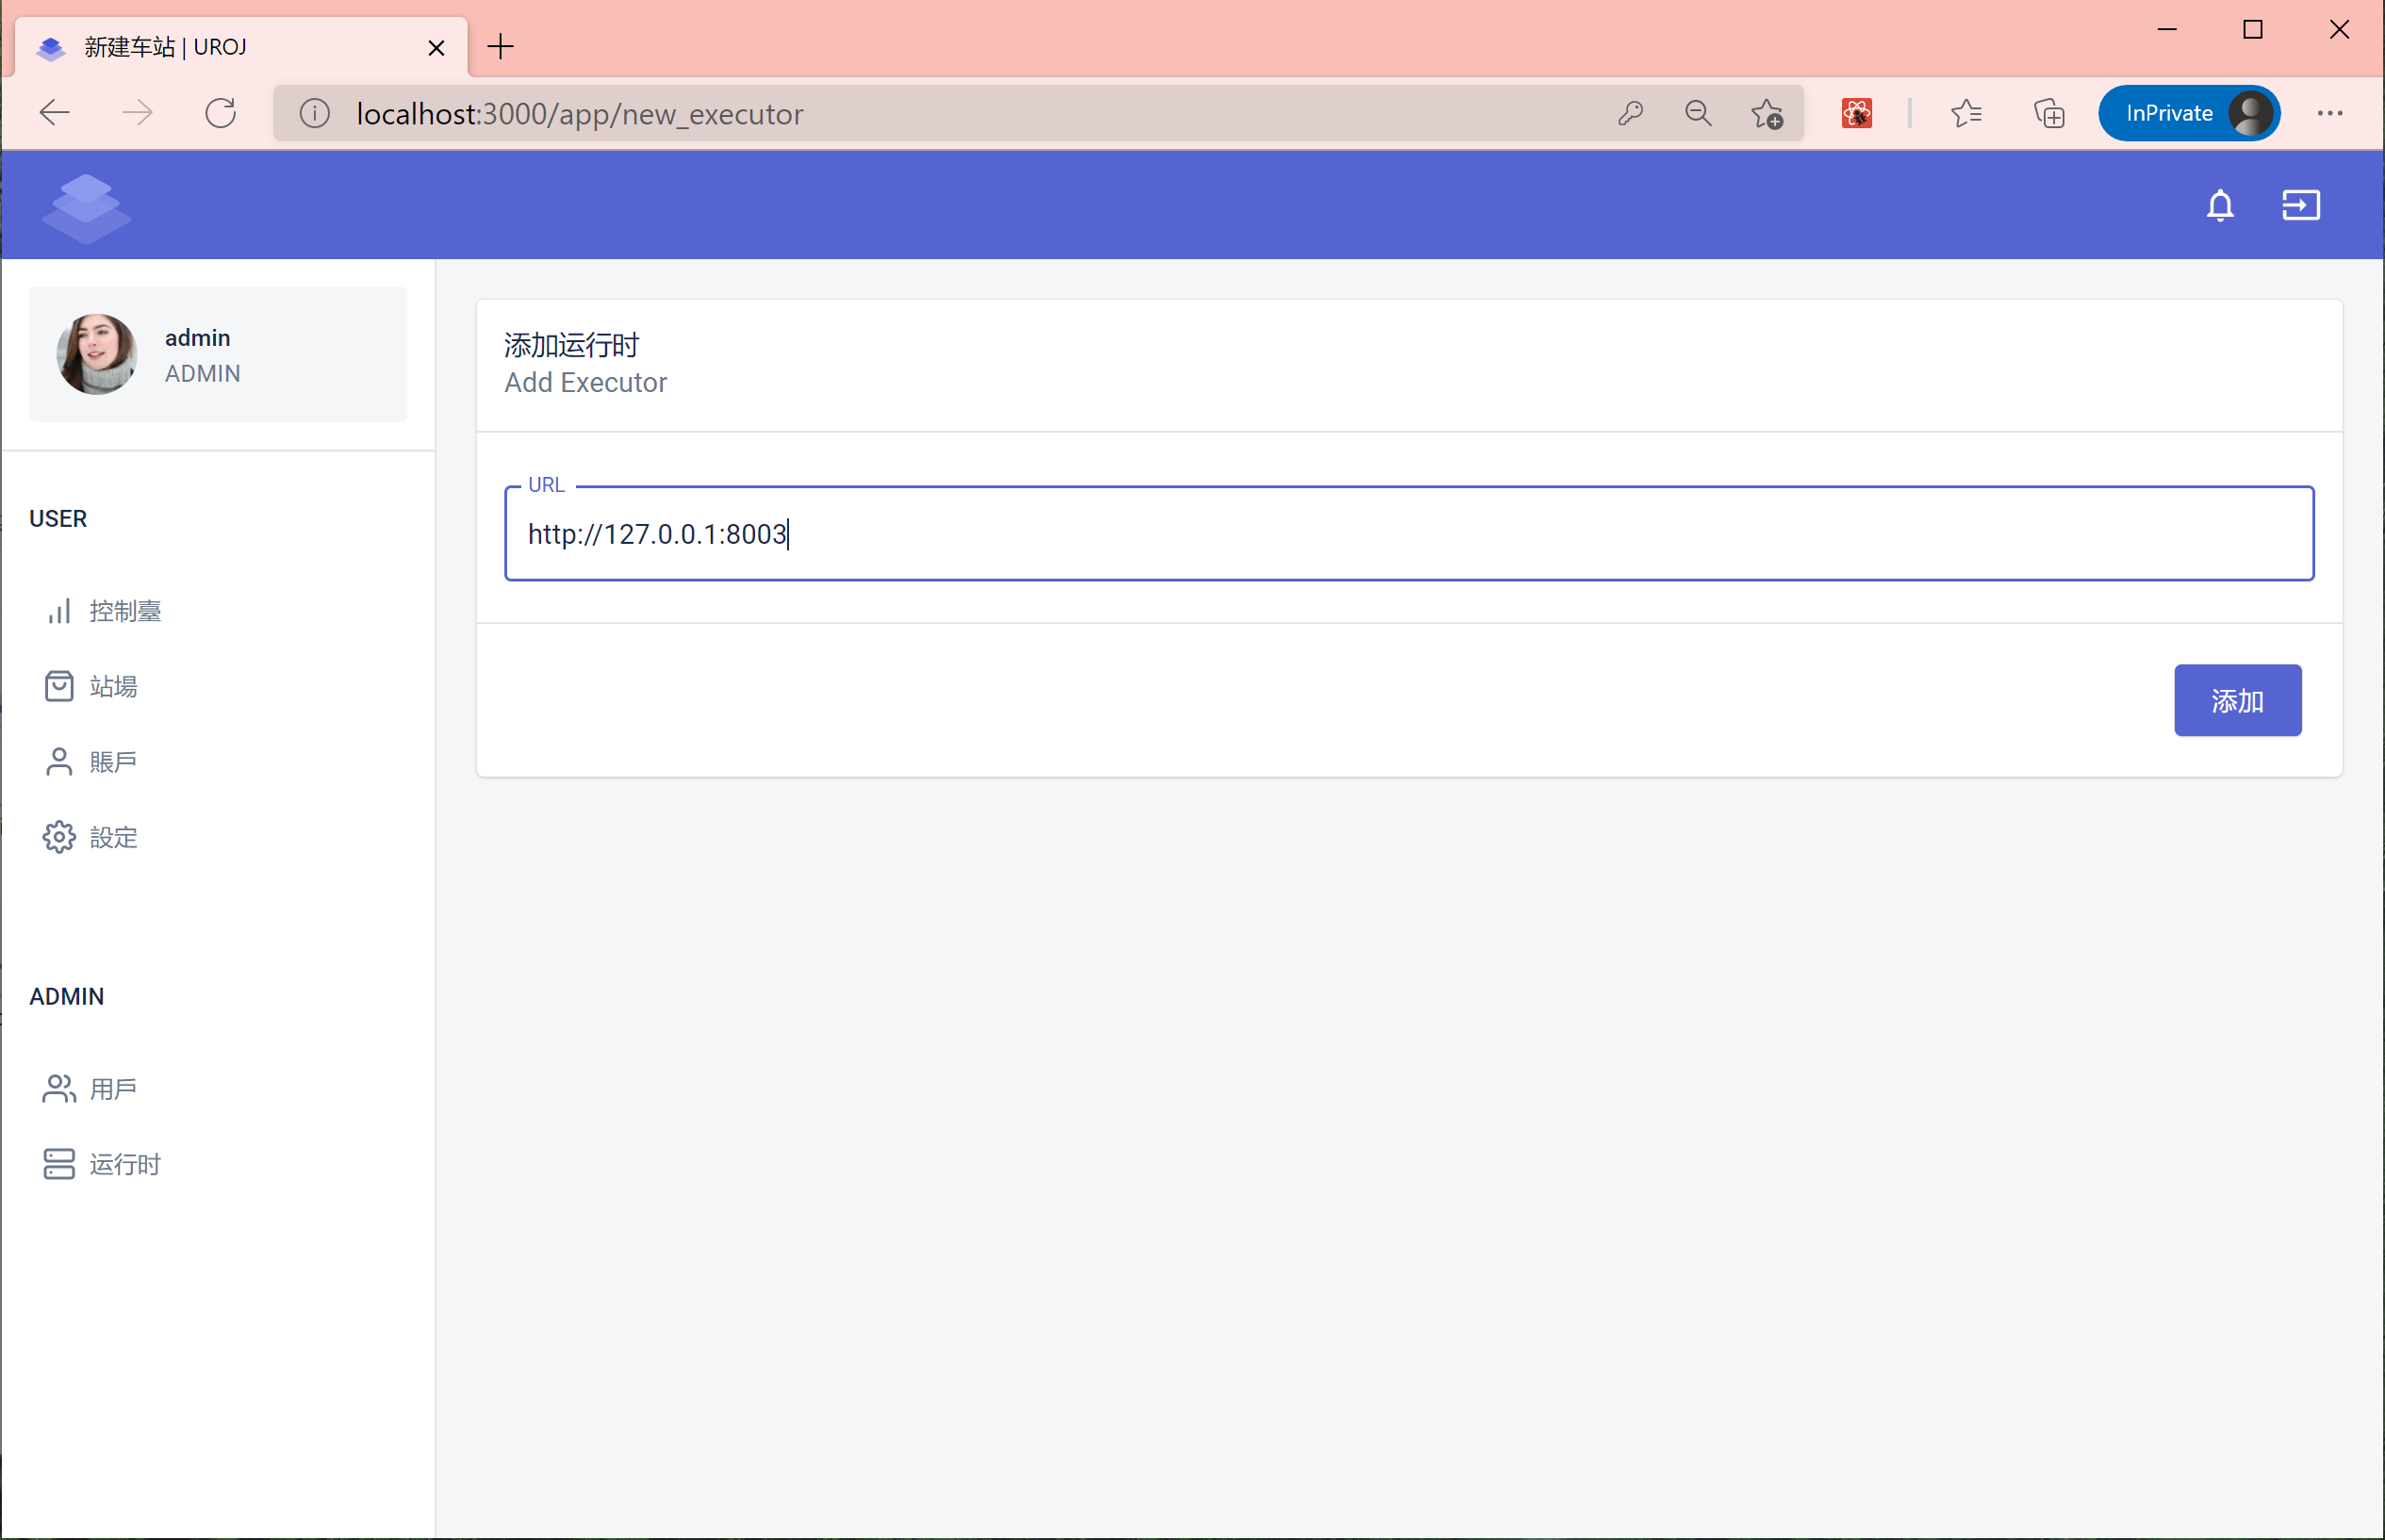
\includegraphics[width=\textwidth]{figures/png/add_exes.png}
  \caption{\label{add_exes}添加运行时}
\end{figure}

\begin{figure}[htbp!]
  \centering
  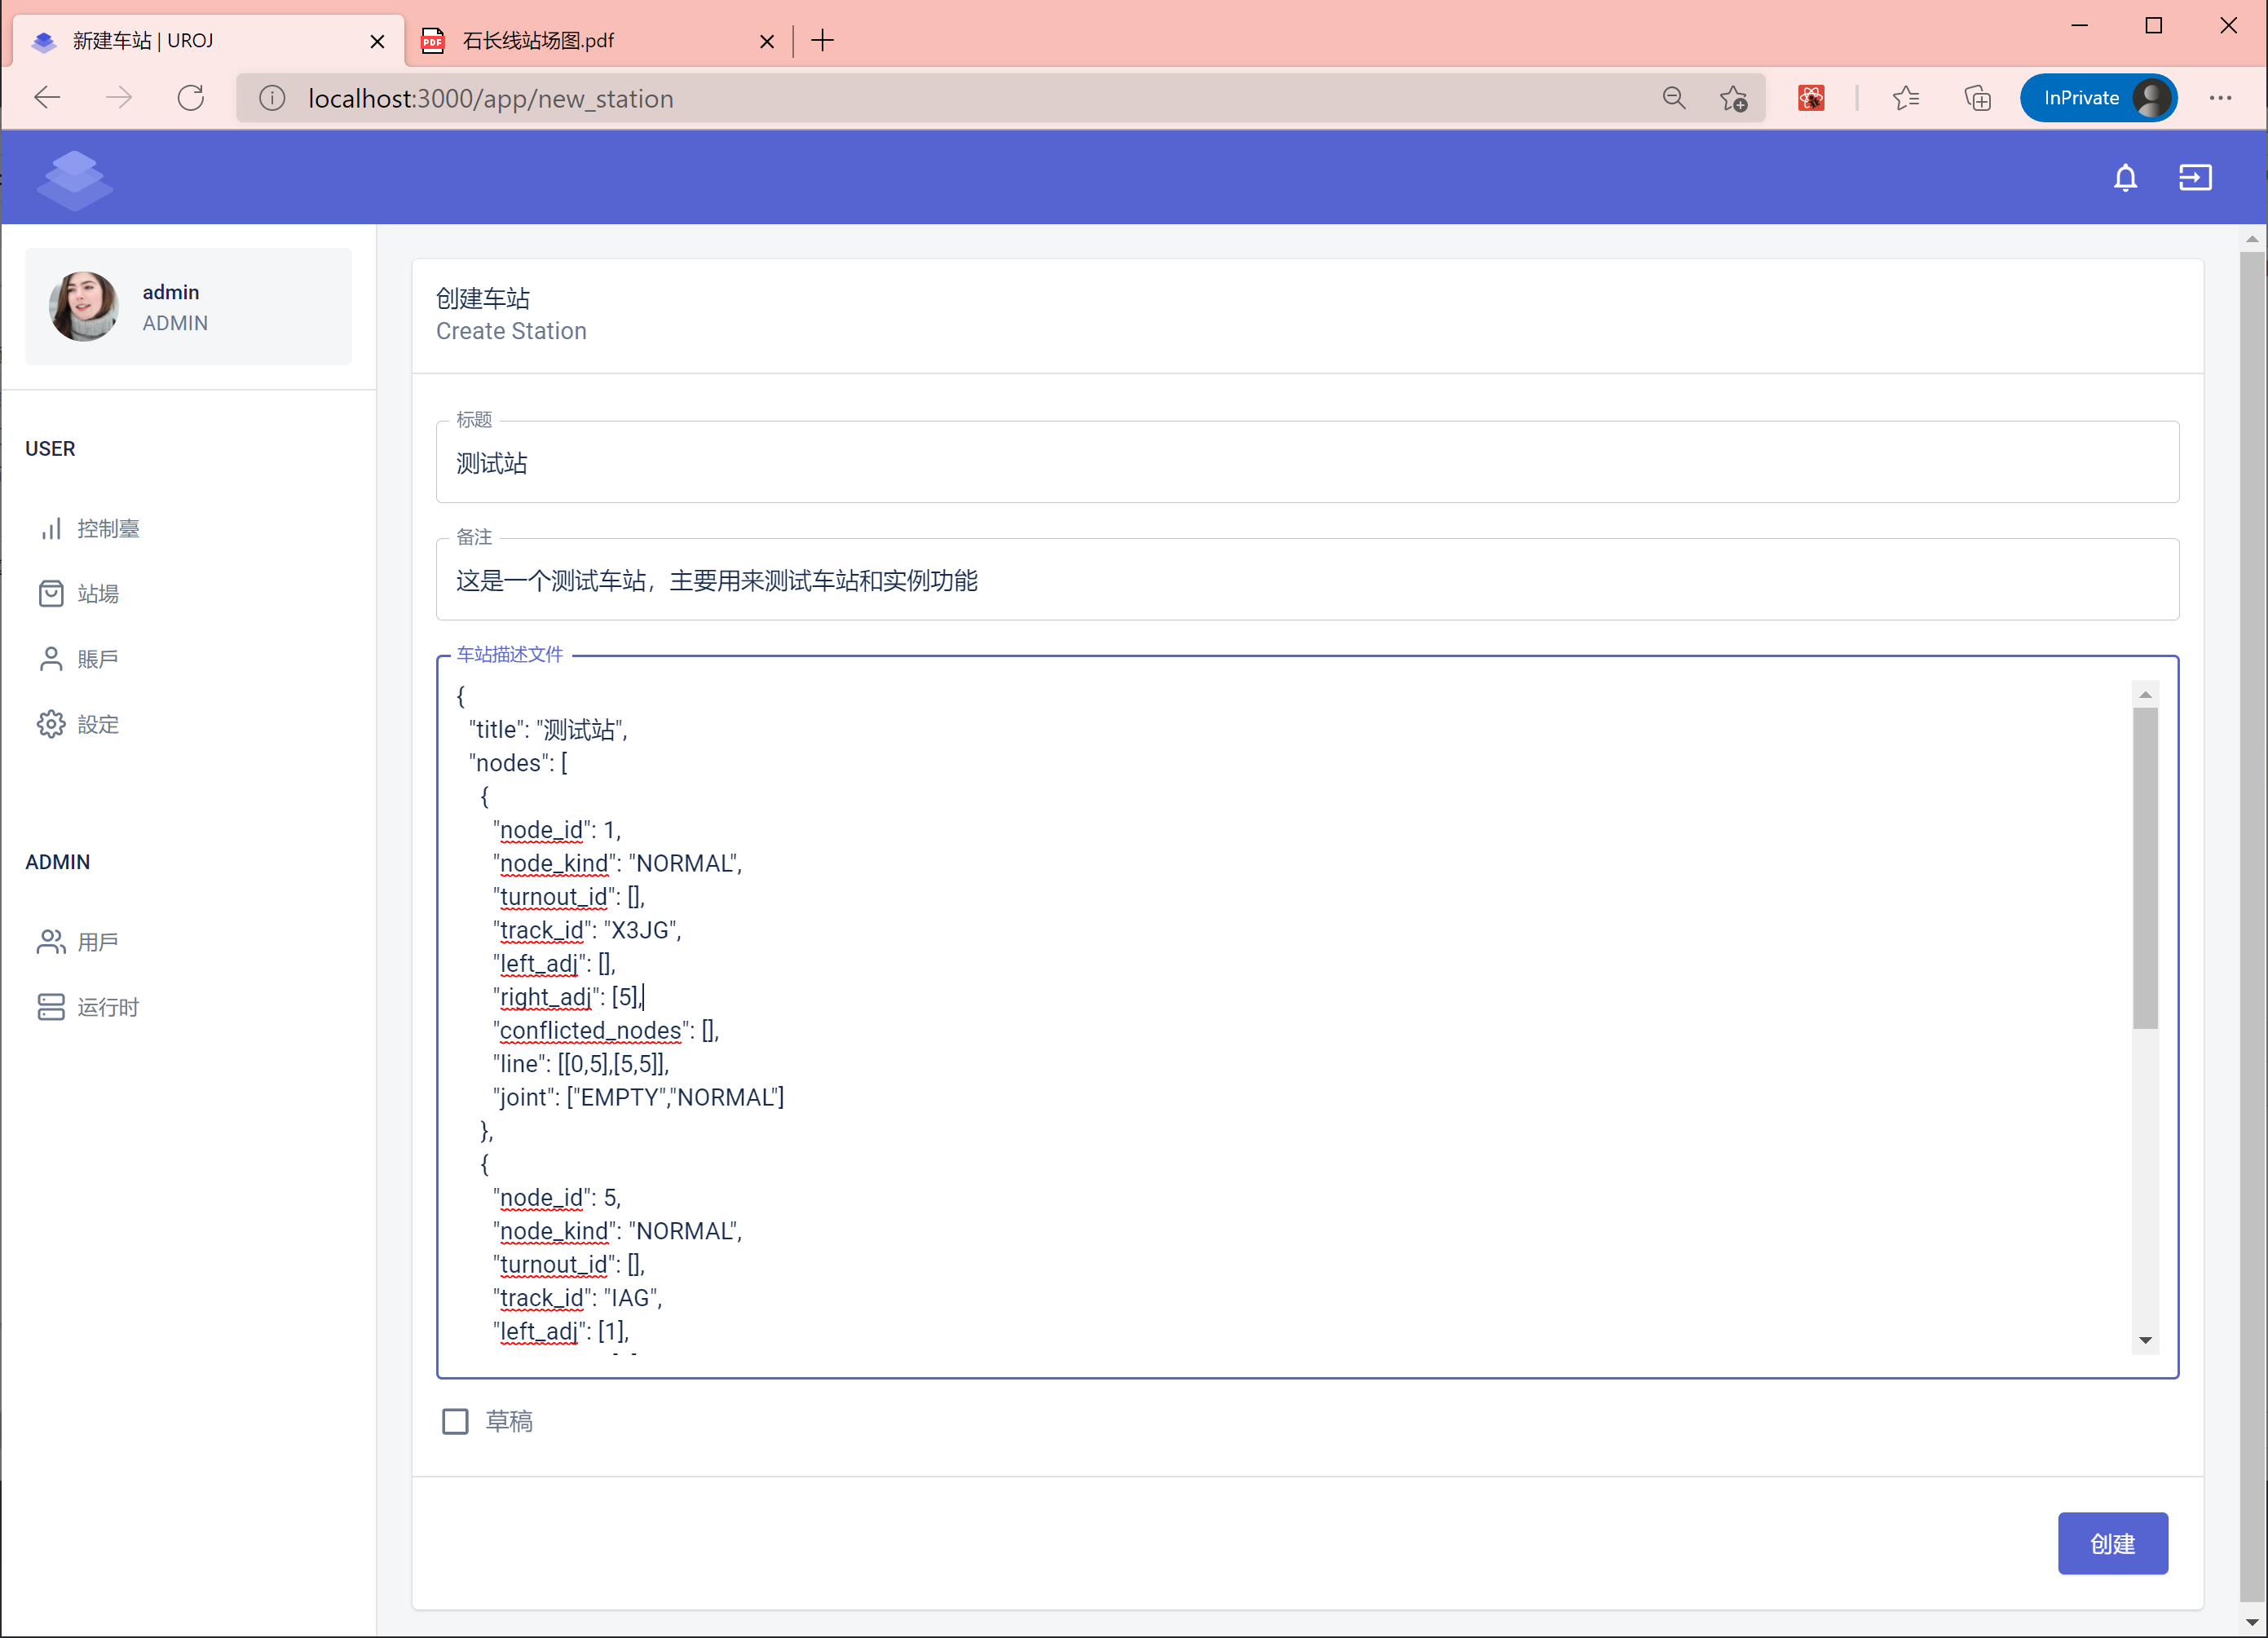
\includegraphics[width=\textwidth]{figures/png/create_sta.png}
  \caption{\label{create_sta}创建车站}
\end{figure}

图\ref{create_sta} 所示的界面是创建车站页面,用户在这里上传车站的相关信息
以及车站描述文件,以新建新车站。

\begin{figure}[htbp!]
  \centering
  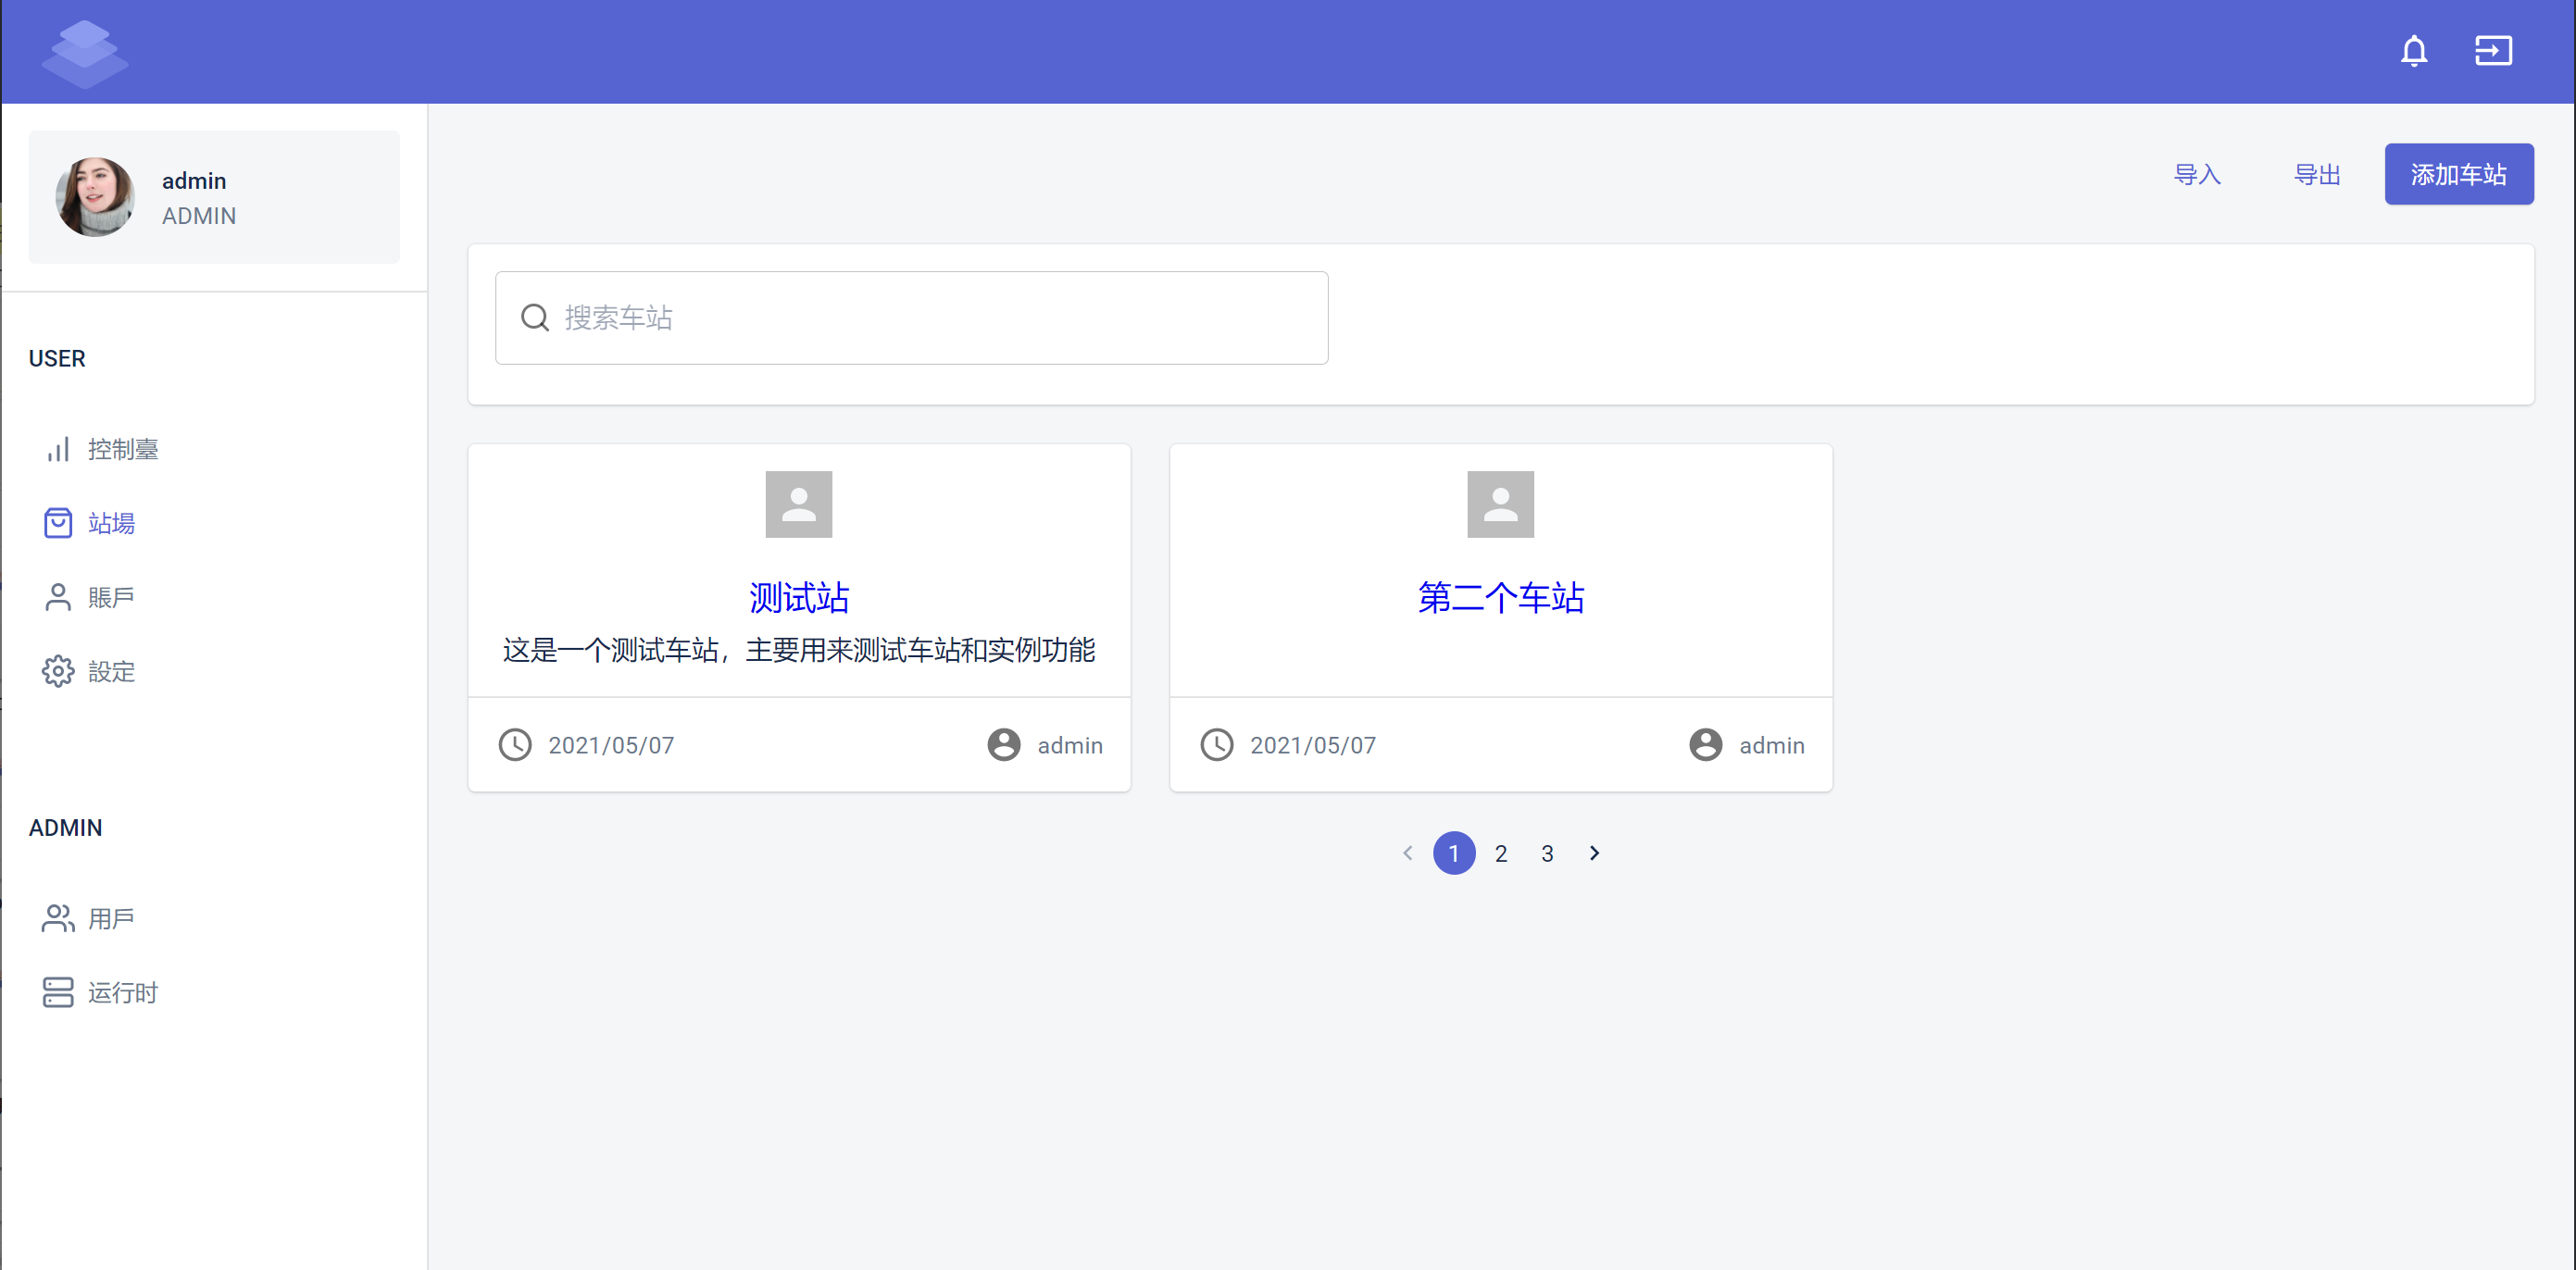
\includegraphics[width=\textwidth]{figures/png/station_list.png}
  \caption{\label{station_list}车站页面}
\end{figure}

图\ref{station_list} 所示页面为车站列表页面,其列出了当前系统中所有
的车站。

\begin{figure}[htbp!]
  \centering
  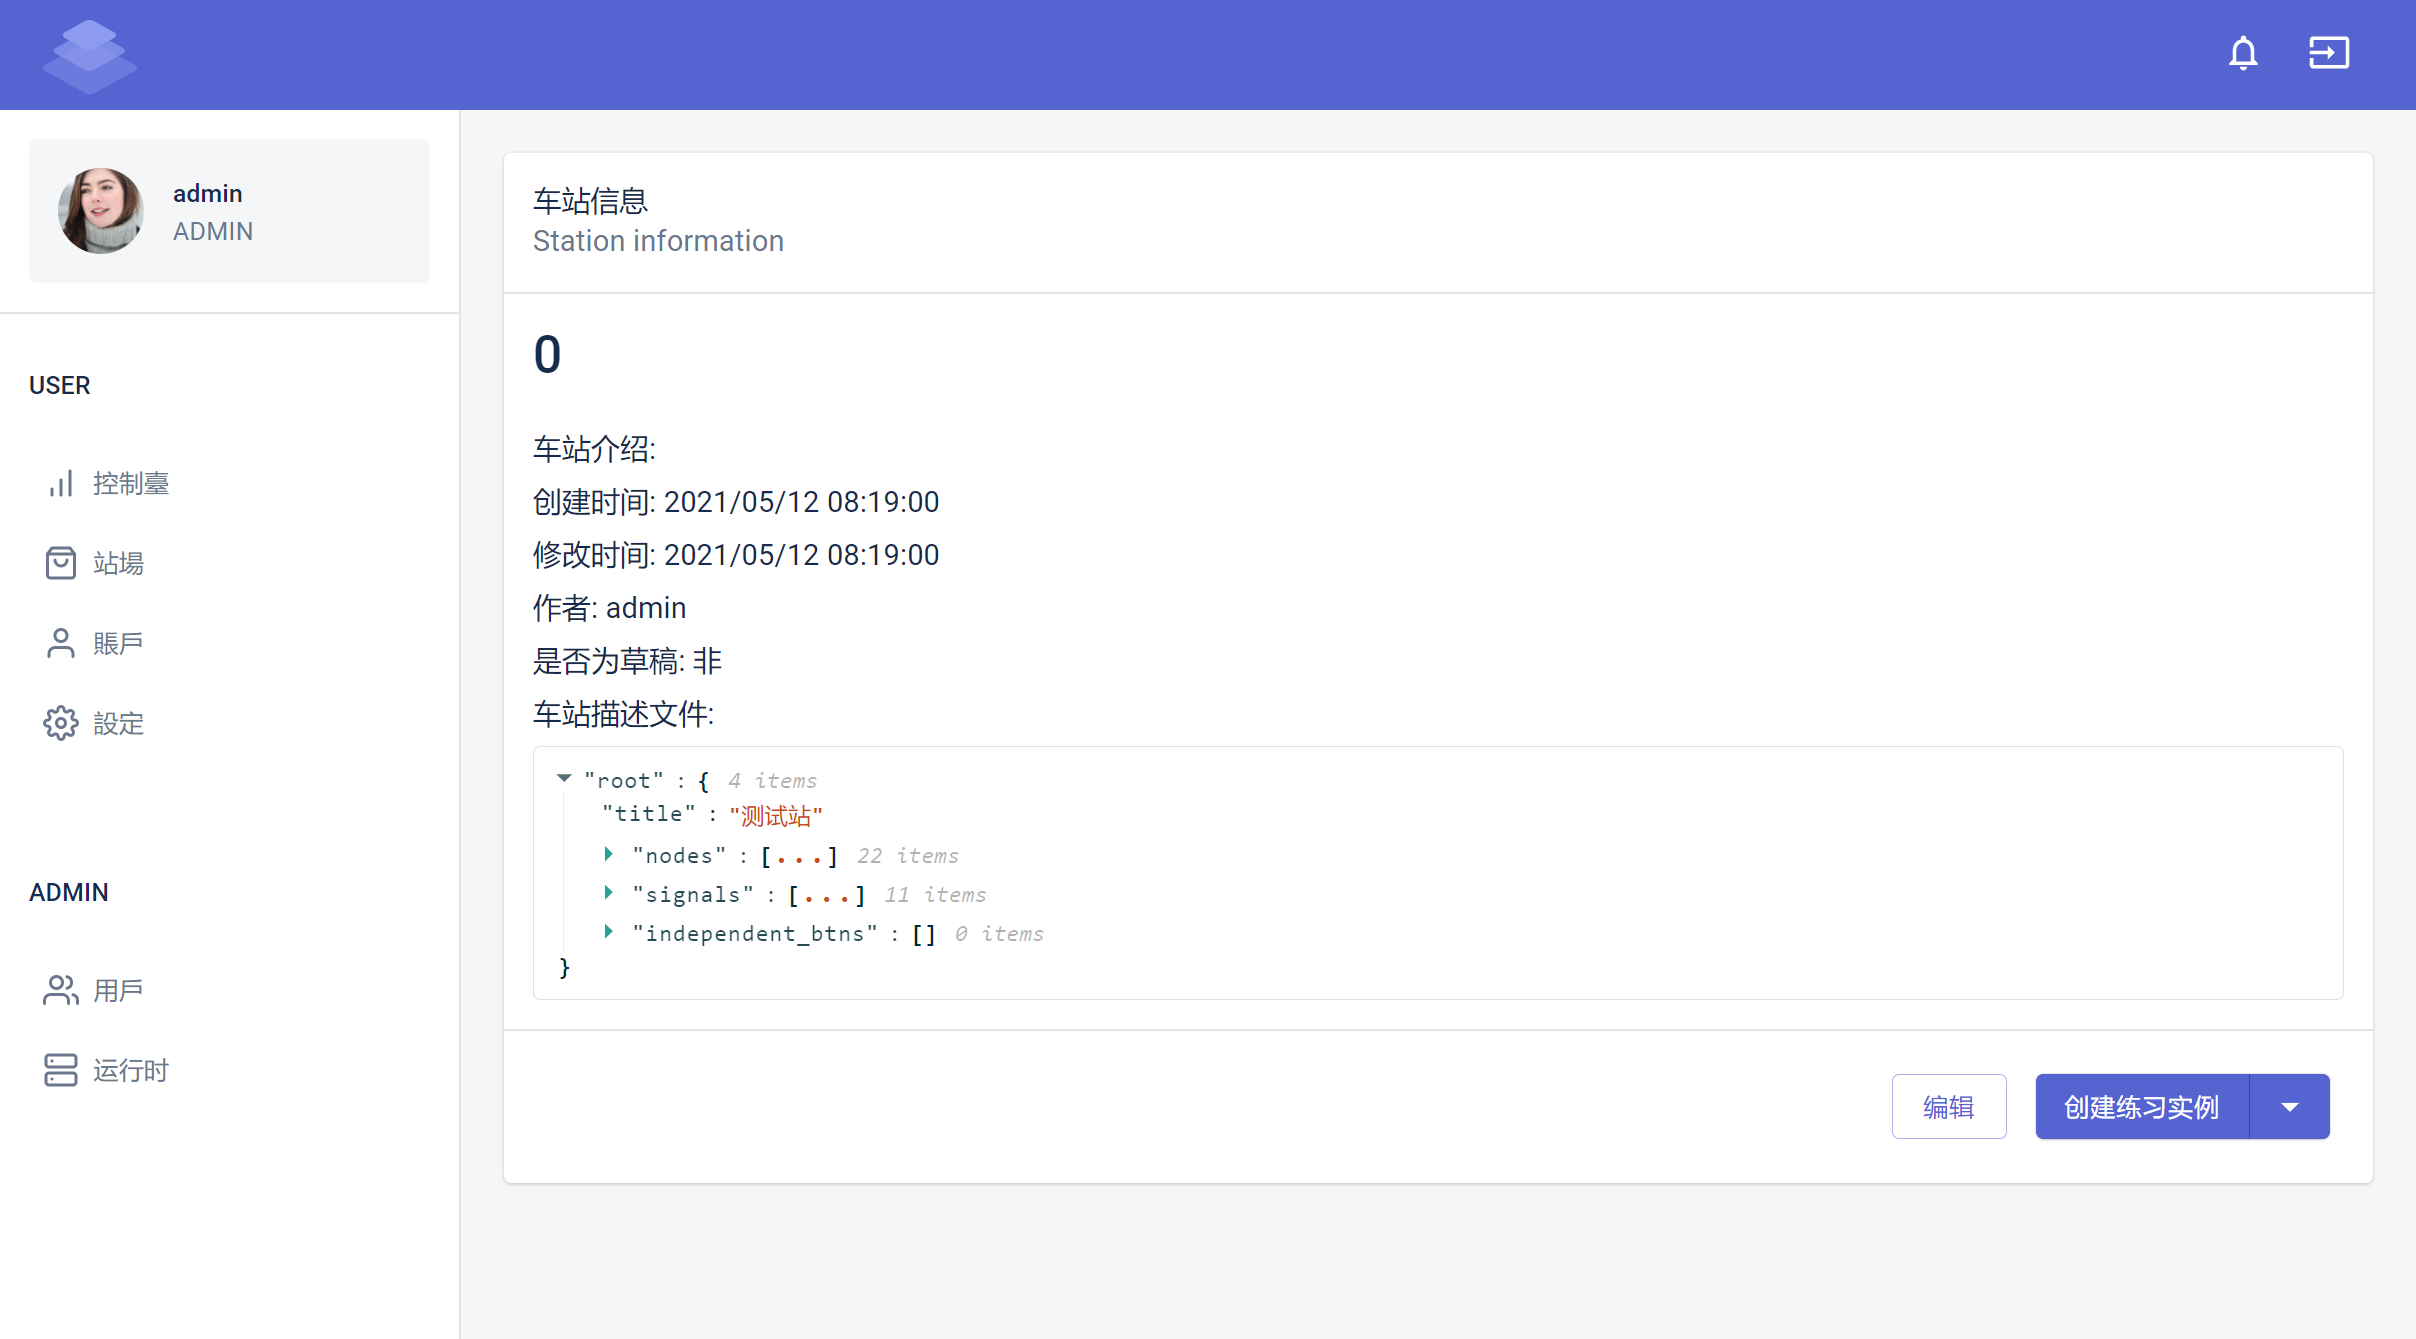
\includegraphics[width=\textwidth]{figures/png/station_info.png}
  \caption{\label{station_info}车站信息查看}
\end{figure}

图\ref{station_info} 所示的页面为车站的详情页面,显示着某个车站的所有信息。
其中为车站描述文件显示称为可交互的树状图,方便用户查看,提升用户体验。

\begin{figure}[htbp!]
  \centering
  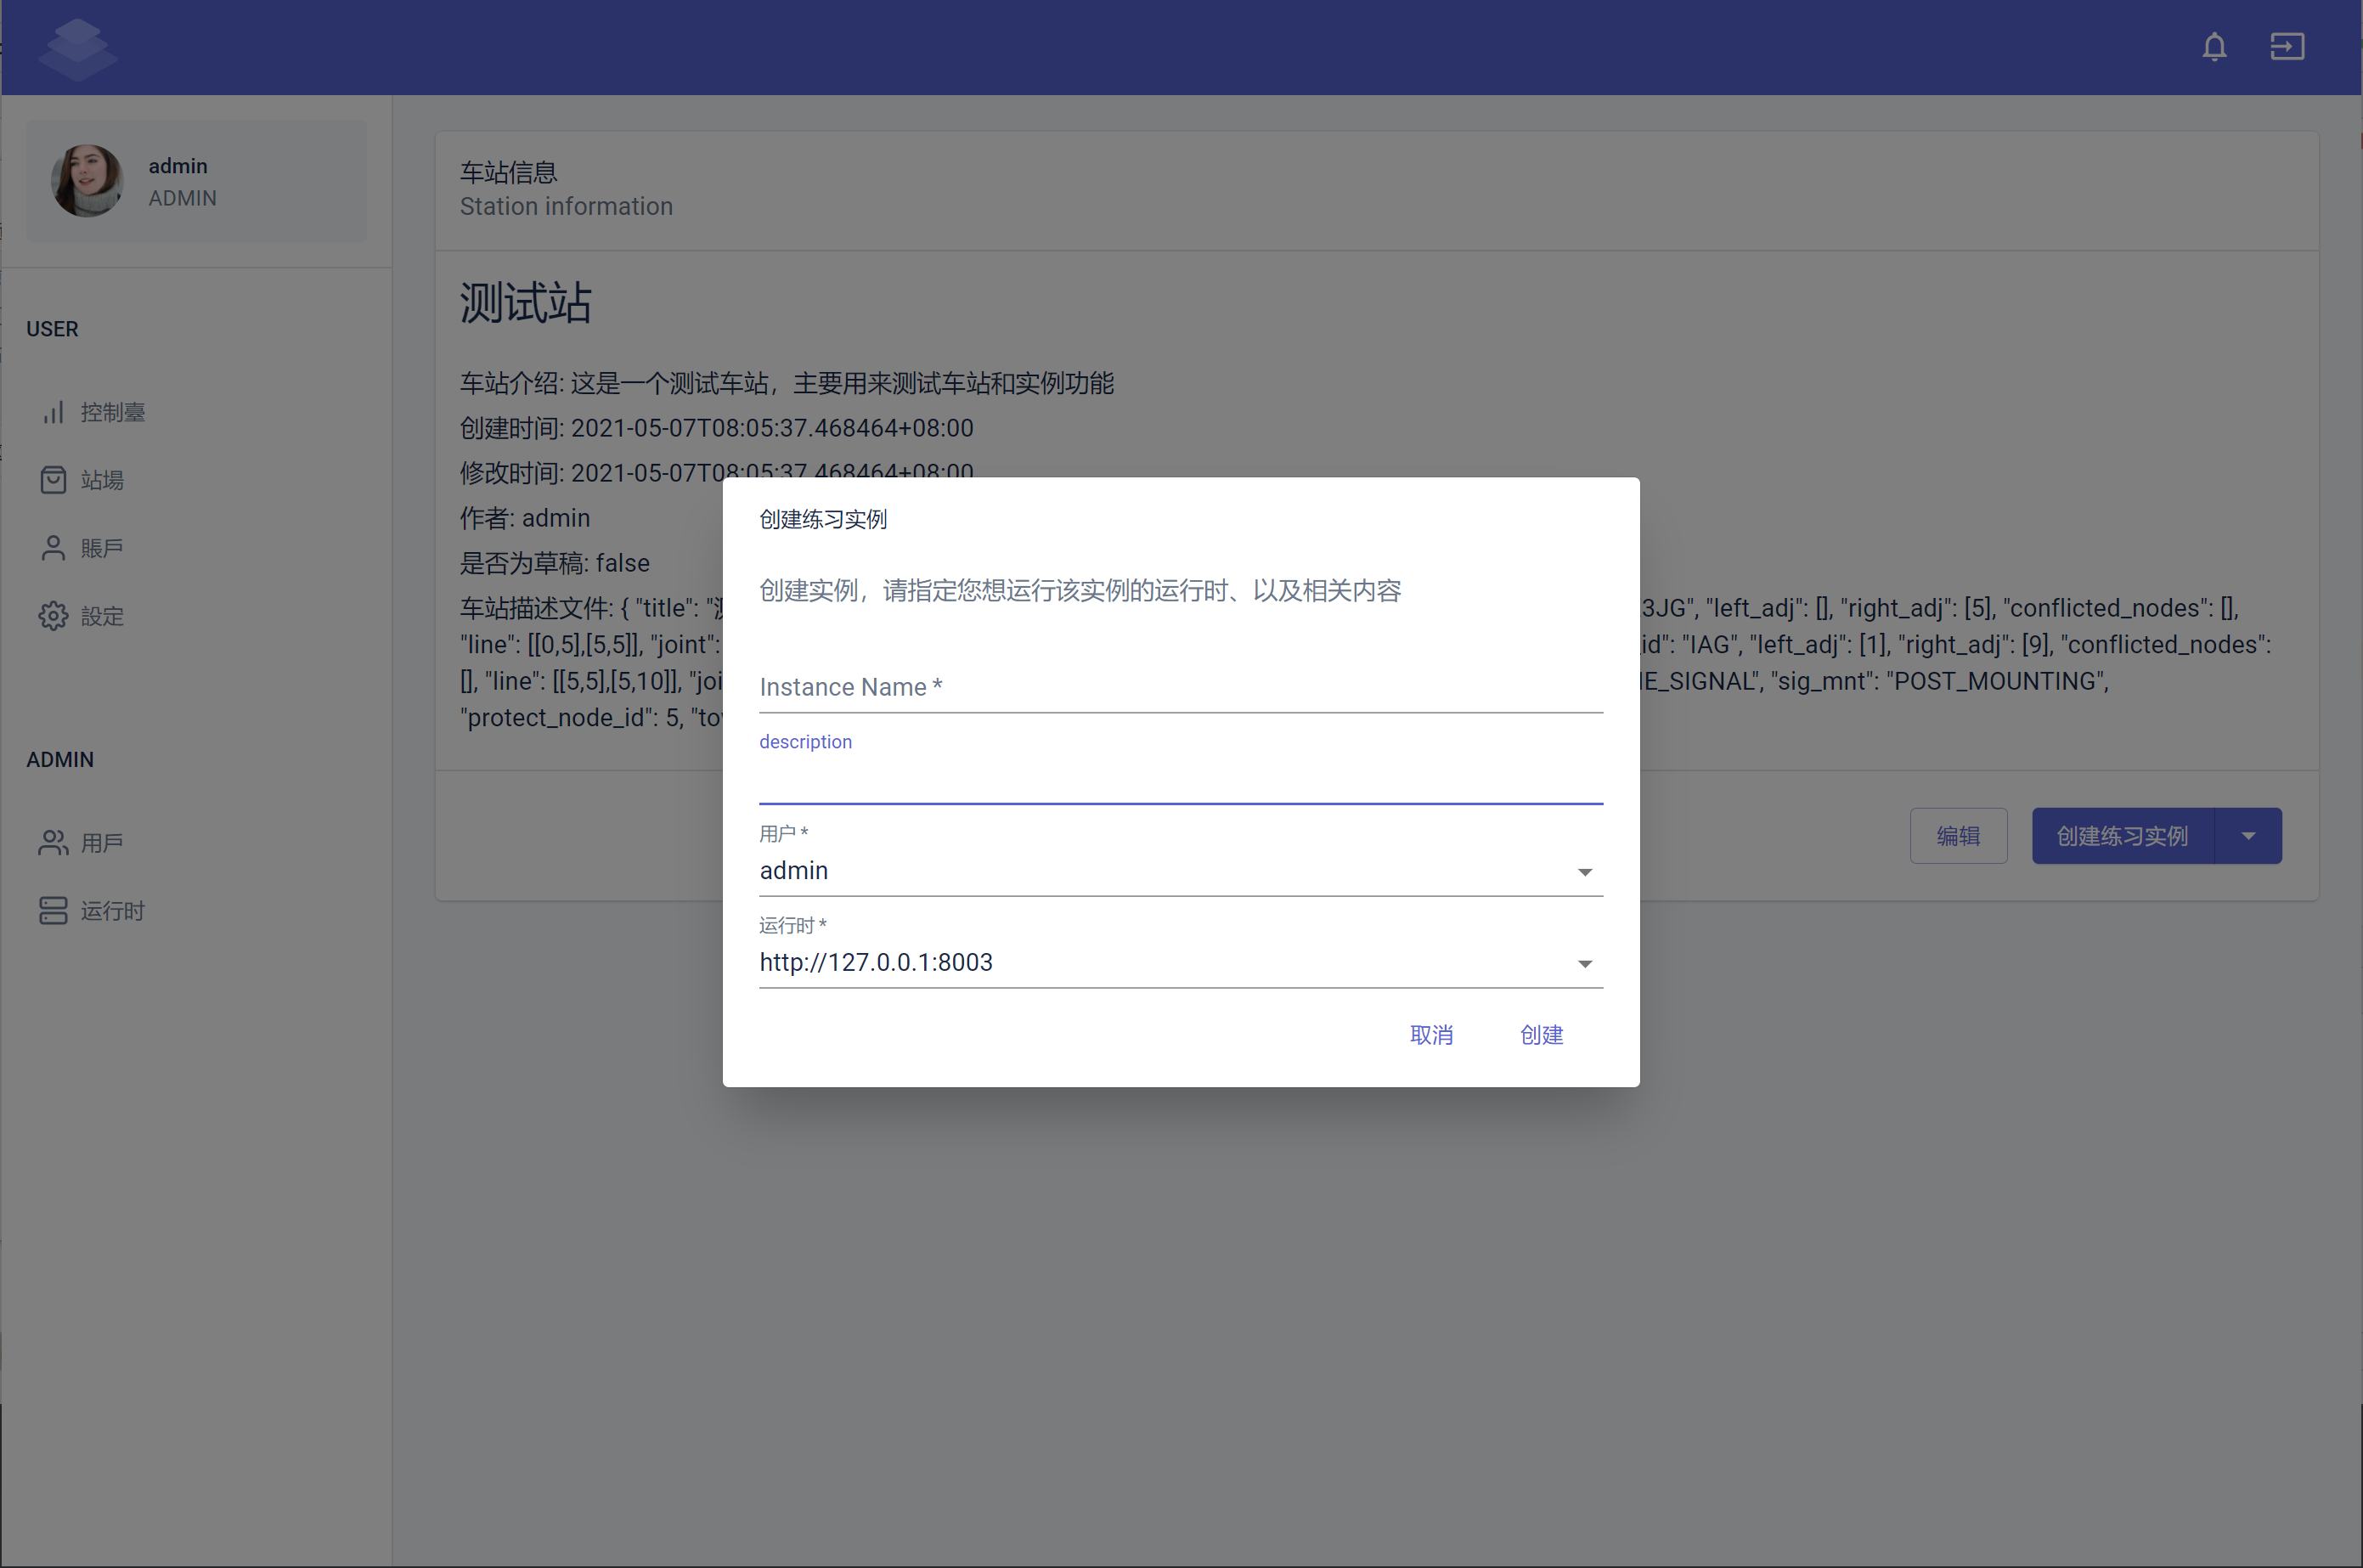
\includegraphics[width=\textwidth]{figures/png/dialog.png}
  \caption{\label{dialog}新建实例对话框}
\end{figure}

点击右下角的按钮后会弹出如图\ref{dialog} 所示的对话框,
用户使用该对话框新建实例。其中用户选单和运行时选单中的数据是从服务器中
获取的所有用户和所有运行时清单,供用户在新建实例时选择。

\begin{figure}[htbp!]
  \centering
  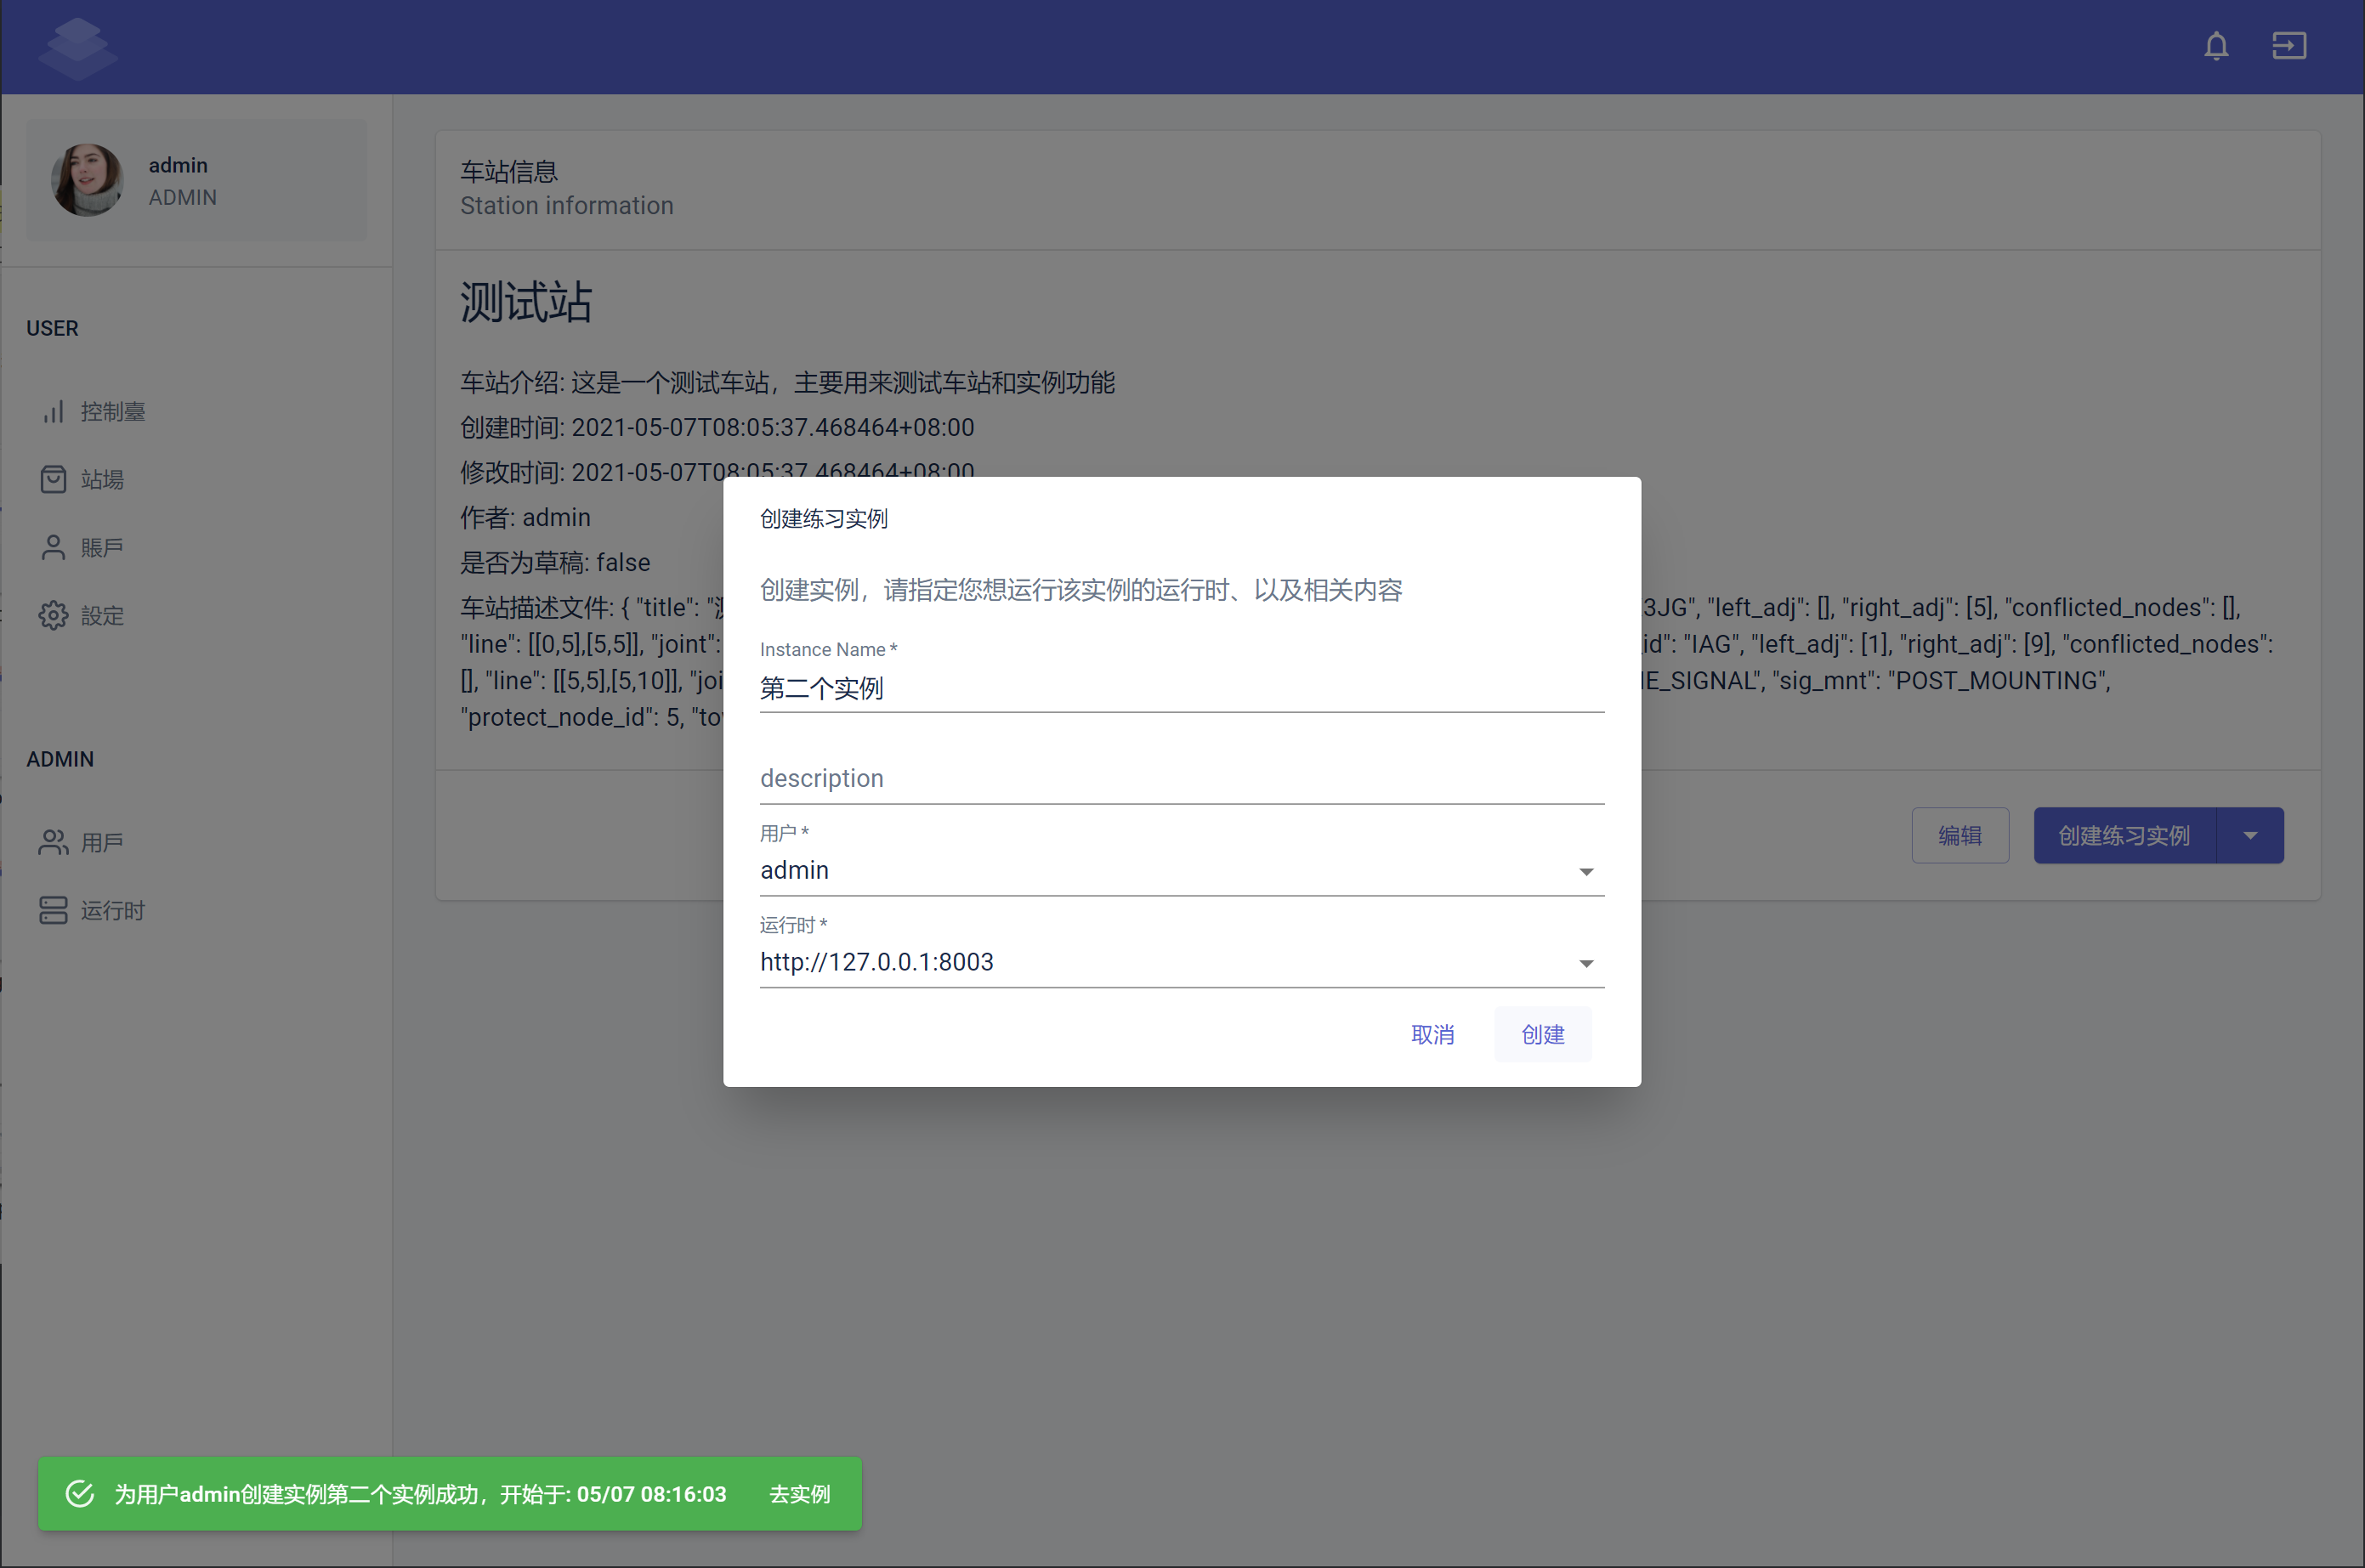
\includegraphics[width=\textwidth]{figures/png/dialog_succ.png}
  \caption{\label{dialog_succ}创建实例成功}
\end{figure}

若新家实例成功,如图\ref{dialog_succ} 所示,
系统会提供用户访问实例的捷径,点击按钮就可以直接访问实例。

\begin{figure}[htbp!]
  \centering
  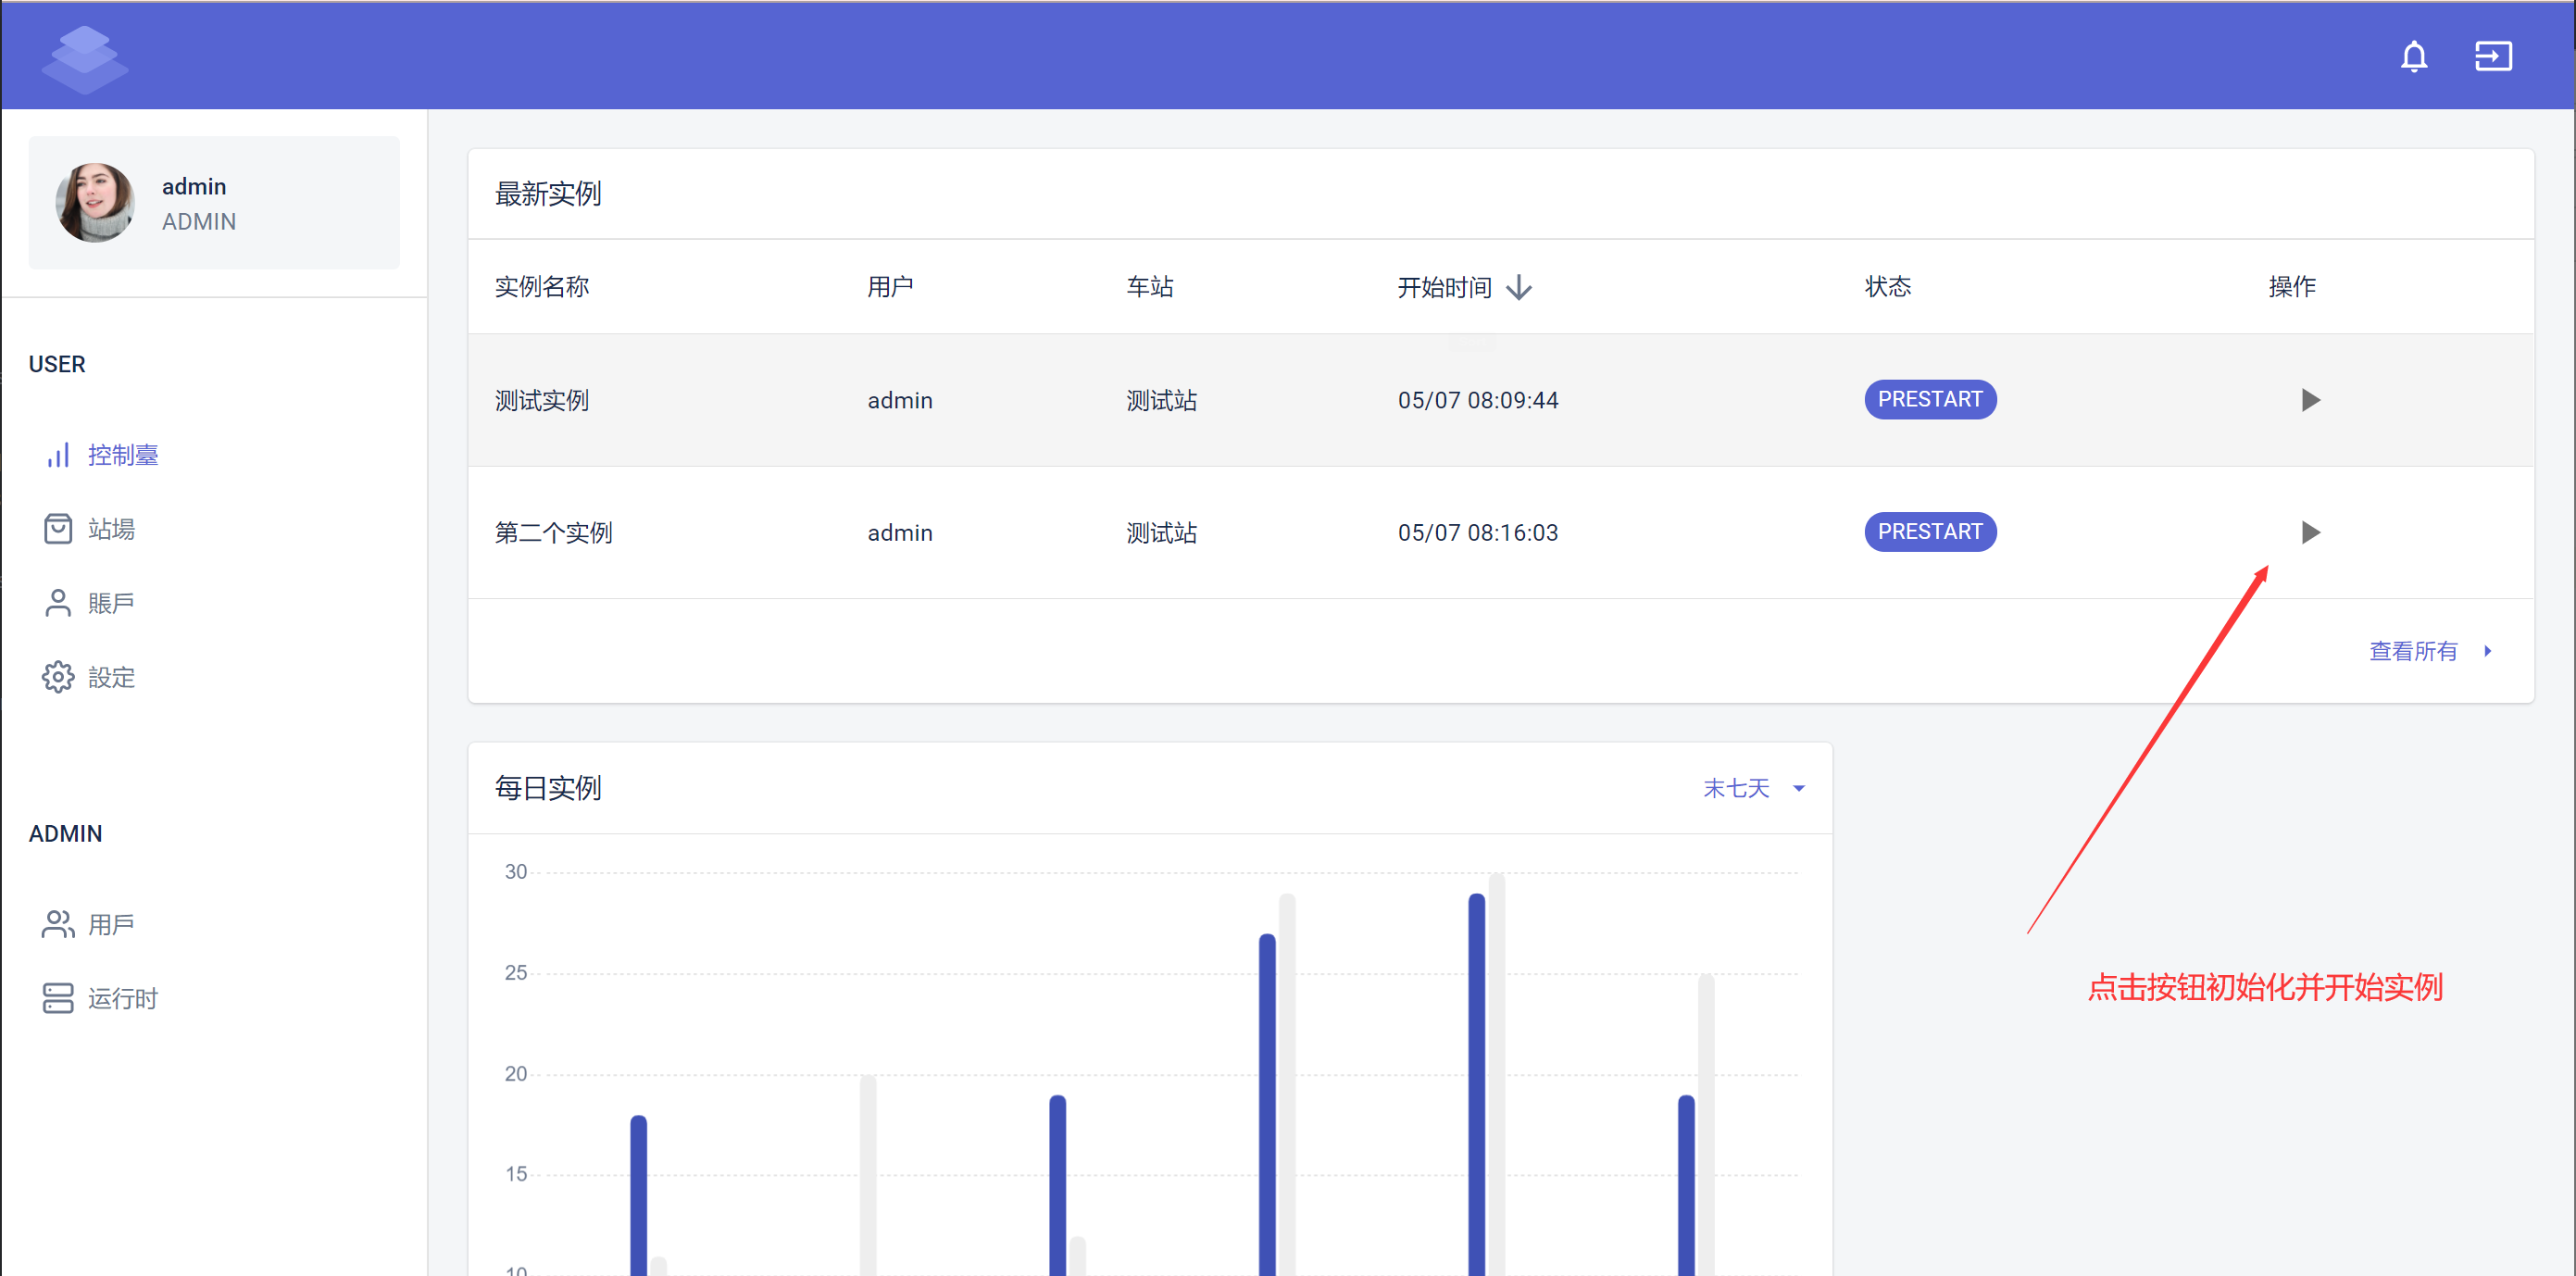
\includegraphics[width=\textwidth]{figures/png/after_create.png}
  \caption{\label{after_create}创建实例后运行实例前}
\end{figure}


\begin{figure}[htbp!]
  \centering
  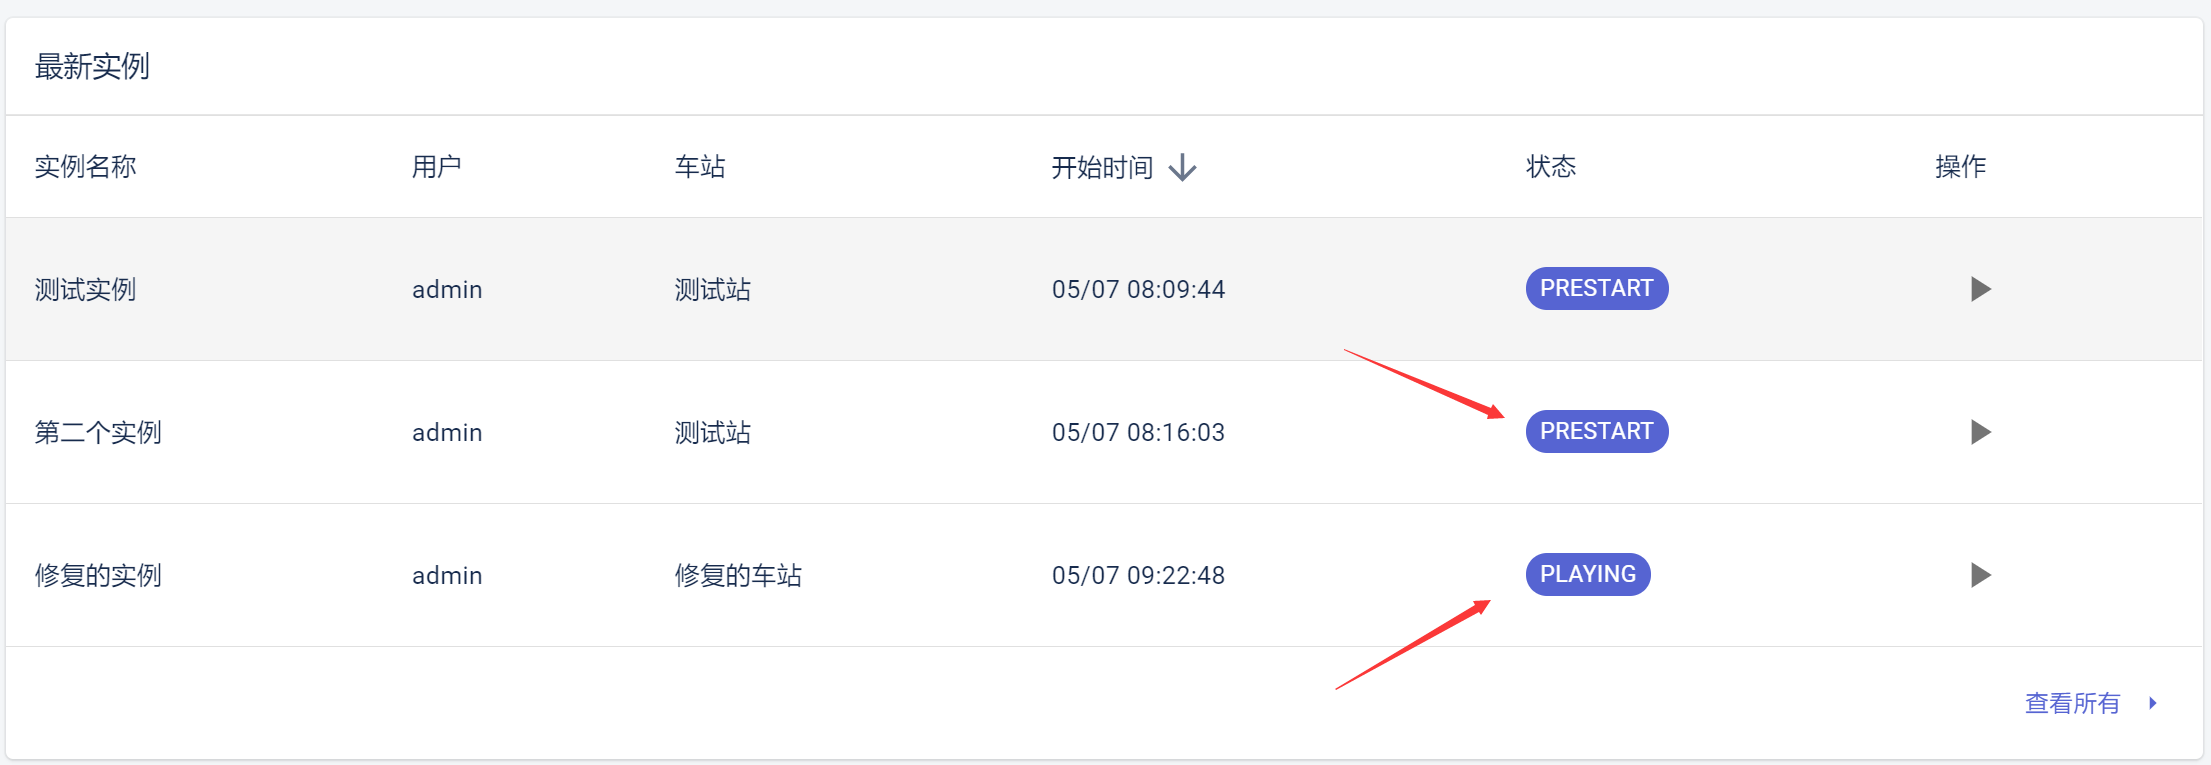
\includegraphics[width=\textwidth]{figures/png/3rd.png}
  \caption{\label{3rd}运行实例后}
\end{figure}

在图 \ref{after_create} 和 \ref{3rd}  中,若当前时间未满开始时间,
则开始的三角按钮不能被按下(图中未体现),也就是前文所述的双重保证。在按下开始按钮后,实例在运行时中被
初始化、运行、实例状态从 PRESTART 变为 PLAYING。表现层的网页
则跳转至实例界面。

% \subsection{实例界面}
